\documentclass[aps,preprintnumbers,onecolumn,amsmath,amssymb,floatfix,pra]{revtex4-1} 

%\documentclass[aps,preprintnumbers,onecolumn,amsmath,amssymb,floatfix,pra]{revtex4} 

%\documentclass[aps,pre,twocolumn,groupedaddress]{revtex4-1}
%\documentclass[a4paper,onecolumn,12pt]{article}
%\documentclass[reprint, amsmath,amssymb,aps,]{revtex4-1}

\bibliographystyle{apsrev4-1}

\usepackage{amsmath}
 \usepackage{amsfonts}
 \usepackage{amssymb}
 \usepackage{graphicx}
 \usepackage{subfigure}
 \usepackage{enumerate}
 \usepackage{verbatim}% for \begin{comment} \end{comment}
 \usepackage{color}
 \usepackage{xcolor}
 \usepackage{bm}
 \usepackage[]{hyperref}
 \hypersetup{
    colorlinks = false,
    linkbordercolor = {red},
    citebordercolor = {green},
}

 \usepackage{epstopdf}

\begin{document}
\title{One-dimensional Classical Gas in a Harmonic Trap with Repulsive Interaction}

\author{
Zhiyu Dong,$^{1,2}$
R. Moessner,$^2$
and Masudul Haque$^{2,3}$}


\affiliation{
  $^1$ Department of Physics and State Key Laboratory of Surface Physics, Fudan University, Shanghai 200433, China\\ 
  $^2$ Max Planck Institute for the Physics of Complex Systems, N{\"o}thnitzer Str.~38, 01187 Dresden, Germany\\
  $^3$ Department of Theoretical Physics, Maynooth University, Co. Kildare, Ireland
}



\date{\today}
 
 
\begin{abstract}

Abstract --  to be written last
   
\end{abstract}

\maketitle


\section{Introduction}

Will write Introduction after everything else is written.  

---------


Stat-mech from the `bottom up'.  Find papers that do the same. 

More detailed citations of breathing mode.  There are also papers on classical breathing mode, e.g.,
by Bonitz.  

Controlled and tunable experimental realizations of confined quantum systems with ultracold atoms
enable nonequilibrium studies of quantum many-body states in novel geometries. A common feature of
many cold-atom experiments is the confinement of a many-body system in a harmonic trap. Trapping
introduces many distinctive features which have no analog in uniform many-body states, including
collective excitations such as breathing modes, dipole modes, and scissors modes. Such trap-related
collective modes have been widely studied both experimentally and theoretically for continuum
systems, especially in the mean-field regime, since the early days after quantum degeneracy was
achieved with trapped atoms \cite{Dalfovo1997}\cite{Jin1996}.

In mean-field perspective, the physics of atom gas in Bose-Einstein Condensation can be described by
the Gross-Pitaevskii equation\cite{Dalfovo1999}\cite{Stringari1996}, where the breathing frequency
for 1D Bose gas is calculated to be $\Omega_{GP}=\sqrt{3}\omega_0$. Meanwhile, the experiment of
Ref.\cite{Haller2009} has found a regime of interactions where the breathing-mode frequency
approaches the Gross-Pitaevskii prediction. However, since mean-field approach which generally omit
quantum fluctuation is successful in this problem, one may wonder how quantum effects play the role
in the breathing mode. Thus, a natural question would be asked is that how breathing frequency is
dependent on interaction for classical gas. Though generated in BEC, the breathing mode phenomenon
is not restricted to BEC. For a classical gas, the breathing mode still can be excited with a
quench. Usually, a good knowledge of the classical version may help us understand the quantum one
better. David Guery-Odelin, Francesca Zambelli, Jean Dalibard, and Sandro Stringari answered this
question in ref.\cite{Guery-Odelin1999}. They used the Boltzmann equation as well as molecular
dynamics simulation to study the monople mode and quarulple mode of the 2-D classical gas in a
harmonic trap. But in that work, the interaction is elastic collision,
i.e. zero-range-infinite-strength interaction. We think introducing a finite range for the repulsive
interaction will definitely enrich the physics in this system which looks simple, thus producing a
different equilibrium and non-equilibrium behaviour. Surprisingly, to the best of our knowledge,
there is no in-depth study of this case. For this reason, more study is necessary.

On the other hand, in a nonquilibrium many-body system, a more intriguing question is about its
thermalization or relaxation property. Thermalization is among the most fundamental processes for a
many-body interacting system. All systems do not thermalize. An example is the Fermi-Pasta-Ulam
paradox [ ] which shows confinement in phase-space so that the system stay non-thermalized for a
long time. A lot of research on thermalization property has been done in other classical
system. Ref.\cite{Tsuchiya2000}\cite{Yawn1997} studied the one dimensional gravitational system with
Lyapunov exponents. Ref.\cite{Jin2013} studied the ring of harmonic oscillators and magnetic moment
by examine the canonical distribution of a subsystem . In our paper, we will also probe the system's
thermalization time scales from the perspective of canonical distribution as well as Lyapunov
exponent.

%With these approaches, we will show that the thermalization time scale manifest a
%competition between total energy and interaction energy, so there is not any singular
%behavior in the thermalization time scales except the trivial divergence at zero
%interaction.


------------------

Breathing frequency, comparisong to quantum case ------ 

Usually, to see the response of quantum gas to a quench, one begin simulation with the ground state
and then suddenly vary some parameter by a little, for instance,
$\omega_0'\rightarrow\omega_0=\omega_0'+\Delta\omega$. In that case, one will observe the radius R
of the cloud oscillating at a certain frequency, which is usually called ``breathing mode".

However, it is quite different in the classical version. Firstly, it is no longer necessary to focus
on ground state. In quantum case, the reason why we care about ground state and low lying
excitations is that BEC occur at low temperature. But in classical case, there is no BEC. So it is
not necessary to focus on low lying excitations in classical case. Besides, since classical limit is
$\hbar\rightarrow 0$, no matter how low the kT is, $\hbar/kT$ is always zero so even in low energy
regime, the classical behaviors could be quite different from the quantum one. Secondly, it is no
longer necessary to vary parameters ``by a little" in the quench. In quantum case, the small quench
$\omega_0'\rightarrow\omega_0=\omega_0'+\Delta\omega$ means the spectrum of Hamiltonian is shifted
slightly, thus one may expect to see some beat phenomenon({\color{red}{?}}). But in classical case,
since $\hbar$ vanishes, no matter how small the quench is, the reason that cause beats in quantum
case no longer work in classical context. Thus it is not necessary to limit ourselves to small
quench.

Let's consider quenching the harmonic potential, i.e.,
$\omega_0\rightarrow\omega_0'=\omega_0+\Delta\omega_0$. We notice that X and P (scaled) are
symmetric for simple harmonic oscillator. In weak interaction limit, the distribution cloud should
be circular when the gas is completely thermalized. The difference between thermalized cloud before
and after quench is that they are circular under different scaling ratio of P and X axis. If we look
at both of them in the phase-space rescaled according to $\omega_0'$, we will find shape of the
cloud before the quench is an ellipse while the final one is a circle.


------------------


This paper is organized as follows: In Section \ref{section:preparation}, we perform a scaling to
reduce the number of parameters of the system. In addition, we briefly observe the ground state and
reveal two dynamically distinct regime of the system, i.e. strong interaction regime and weak
interaction regime. In Section \ref{section:breathing frequency}, we evaluate the breathing
frequency according to its mechanism, and compare that with our numerical simulation
result. Besides, we also introduce a rotating frame method of treating this problem, which is a
convenient tool to analyze simple harmonic systems. In section \ref{section:Thermalization}, we
focus on the thermalization property. We first examine the canonical distribution of energy to find
out the threshold of thermalization, i.e. under what parameter the thermalization time scale is very
large. In the end of this section, we measure the Lyapunov Exponent to quantify the time scales and
confirm the former discussion. Then we point out that there are two kind of thermalization behavior
that could be measured in this system, one is about energy distribution while another is about shape
of cloud in phase-space. Since here we find two sense of ``thermalizing", we will redefine our terms
-- When a system's energy distribution goes to equilibrium, we still call it ``thermalized".  But
when a system's distribution in phase-space goes to equilibrium, we call it ``relaxed" to distiguish
it from ``thermalized". So in section \ref{section:Shape} we actually study the ``thermalizing" of
the shape of the cloud in phase-space, or the ``relaxation" behavior of the system. There we
discovered a long-lasting mode, which turns out to be a quadruple mode in phase-space.




\section{The model and its equilibrium properties}\label{section:preparation}

\subsection{Model and Scaling}

Our model for the interacting classical gas involves particles with a simple finite-range repulsive
interaction.  Two particles repel each other whenever they are within a distance $\sigma$ from each
other.  The force of repulsion is a constant, $F_0$, within this distance and zero when the distance
is larger. 
%
\begin{equation}
\Big| F(|x|) \Big| ~=~ \begin{cases}
F_0  &\quad |x|<\sigma\\
0  &\quad |x|>\sigma
\end{cases}
\label{eq:preparation1}
\end{equation}
where $|x|$ is the distance between two particles.  This equation describes the magnitude of the
interparticle force; the direction is always repulsive.

The gas contains $N$ such identical particles, each of mass $m$, in a harmonic trap.  The
Hamiltonian describing the gas is 
\begin{equation}
H=\frac{1}{2}m\omega_0^2\sum_{i}x_i^2+\frac{1}{2}m\sum_i
v_i^2+\sum_{\left|x_i-x_j\right|\textless\sigma}F_0\left(\sigma-\left|x_i-x_j\right|\right)
\label{eq:preparation2}
\end{equation}
%
It is useful to rescale the quantities.  We will measure distance, time, energy and force in units
of $\sigma$, $1/\omega$, $m\omega_0^2\sigma^2$ and $m\omega_0^2\sigma$ respectively:
\begin{equation} \label{eq:transform}
  \tilde{x_i} = \frac{x_i}{\sigma}\ , \quad 
  \tilde{H} = \frac{H}{m\omega_0^2\sigma^2}\ ,  \quad \tilde{t} = \omega_0t \ ,  \quad 
\tilde{F_0} = \frac{F_0}{m\omega_0^2\sigma}\ .
\end{equation}
%
Eq.~\ref{eq:preparation2} is then rewritten as
\begin{equation}
  \tilde{H} =
  \frac{1}{2}\sum_{i}\tilde{x_i}^2
  + \frac{1}{2}\sum_i\left(\frac{d\tilde{x}_i}{d\tilde{t}}\right)^2 
  + \sum_{\left|\tilde{x_i}-\tilde{x_j}\right|\textless
    1}\tilde{F}_0\left(1-\left|\tilde{x_i}-\tilde{x_j}\right|\right)  
\end{equation}
%
Through this rescaling, we have reduced the number of the parameters in our model to three: the
energy $\tilde{H}$, the interaction strength $\tilde{F_0}$, and the number of particles $N$.  The
rescaling is equivalent to setting $\sigma$, $\omega_0$ and $m$ to $1$; this is what we do in our
numerical simulation.  In the rest of this paper, we will use ``E" and ``$F_0$" to denote the
reduced versions $\tilde{H}$ and $\tilde{F_0}$.

We will be concerned with the size of the cloud.  We quantify the size through the root-mean-square
of particle positions $\left\lbrace x_i\right\rbrace$, 
\begin{equation}
R\equiv\left(\overline{x_i^2}\right)^\frac{1}{2} \, ,
\label{eq:def_of_R}
\end{equation}
and refer to this quantity as the `radius' or `cloud radius'.

In the dilute gas limit, there are few or no interactions occuring at most times.  Thus the energy
$E$ is dominated by the trap energy, i.e., $E\approx m\omega_0^2\sum_{i}x_i^2= Nm\omega_0^2R^2$, or,
in our units,
\begin{equation}
  E\approx NR^2 \, .
  \label{eq:E_and_R}
\end{equation}
This is a good approximation at large $F_0$ because, for very large interactions, the particles
behave has hard rods which bounce off each other very rapidly, so that at most instants one can
expect no collisions to be taking place.  It is also expected to be a good approximation at very
small $F_0$ since we can then simply neglect the interaction energy.  Thus, we will use this as a common
estimate for $R$ in terms of the energy. 


%%%%% FIGURE %%%%% FIGURE %%%%% FIGURE %%%%% FIGURE %%%%% 
\begin{figure}[tbhp]
\centering
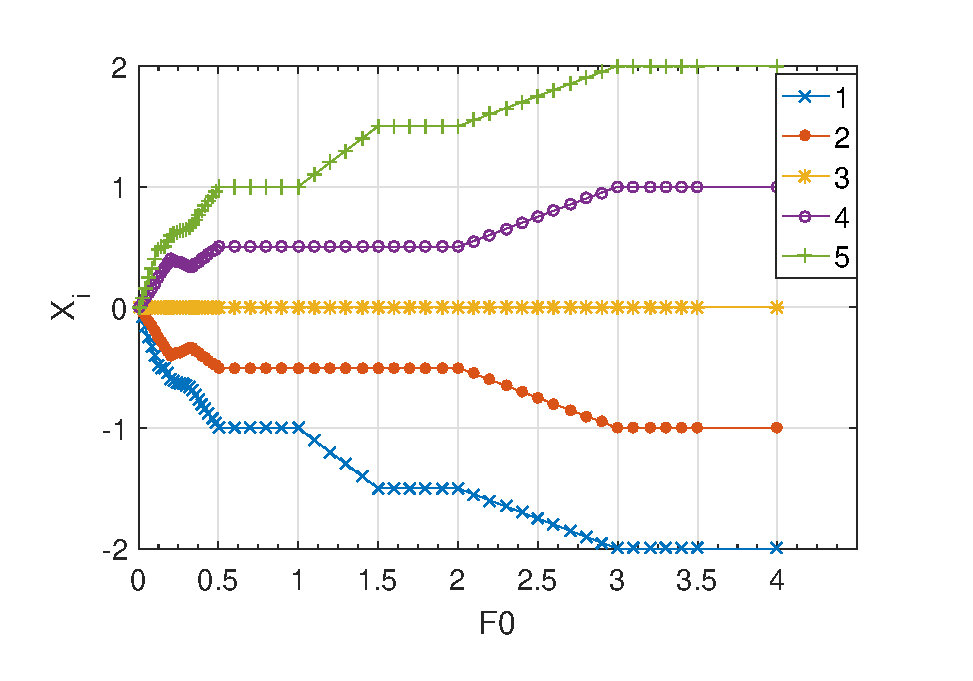
\includegraphics[scale=0.6]{ZhiyuPictures/N=5_GS_pre_2_rev.eps}
\caption{The ground state of a system with $N=5$ particles, shown via the positions of each
  particle, labeled 1 through 5.  At large interactions, the particles position themselves just
  outside the range of interactions of the neighboring particles.}
\label{fig:GS1}
\end{figure}
%%%%% FIGURE %%%%% FIGURE %%%%% FIGURE %%%%% FIGURE %%%%% 




\subsection{Ground states}

The lowest-energy state of the system has zero kinetic energy; in this state the particles find
stationary positions which minimize the trap (potential) and interaction energies.  The trap
potential tries to squeeze the particles towards the trap center, while the interaction tries to push
them apart.

Because of the `Heaviside theta' form of our interaction, at large enough interactions (large $F_0$)
the particles are spaced exactly at distance equal to the range $\sigma$, which is distance $1$ in
our rescaled units.  The interaction is then effectively a `hard-core' interaction.

At very small $F_0$, the particles in the ground state are close enough to the trap center that each
particle interacts with every other particle.  Equating the interaction force due to all the other
particles with the trapping force, one finds that the position of the $i$-th particle is
\begin{equation}
x_i ~=~ \frac{2F_0}{m\omega_0^2} \left( i - \frac{N+1}{2} \right) ~=~ 2F_0 \left( i - \frac{N+1}{2} \right)
\end{equation}
where the particles are labeled $i=1$ to $i=N$ from left to right.  Thus the particles are
equidistant in this regime.  In this `solid'-like state, the low-lying
excitation involves independent oscillation of the particles around their equilibrium position.

In this regime, the distance between the leftmost and rightmost particles is at most $\sigma=1$.
Thus, this situation extends up to $F_0 = \frac{1}{2(N-1)}$.  For the $N=5$ case shown in Figure
\ref{fig:GS1}, this behavior is seen up to $F_0 < 1/8$.


In Figure \ref{fig:GS1}, we can see this crossover from the ``solid-like'' limit (left) to the
``hardcore gas'' limit (right).  In between, there is a rich staircase-like structure, as the
particles attempt to minimize the interaction by being at distance $>1$ from as many other particles
as is compatible with the trap energy.


\subsection{Phase space snapshots}


%%%%% FIGURE %%%%% FIGURE %%%%% FIGURE %%%%% FIGURE %%%%% 
\begin{figure*}[h]
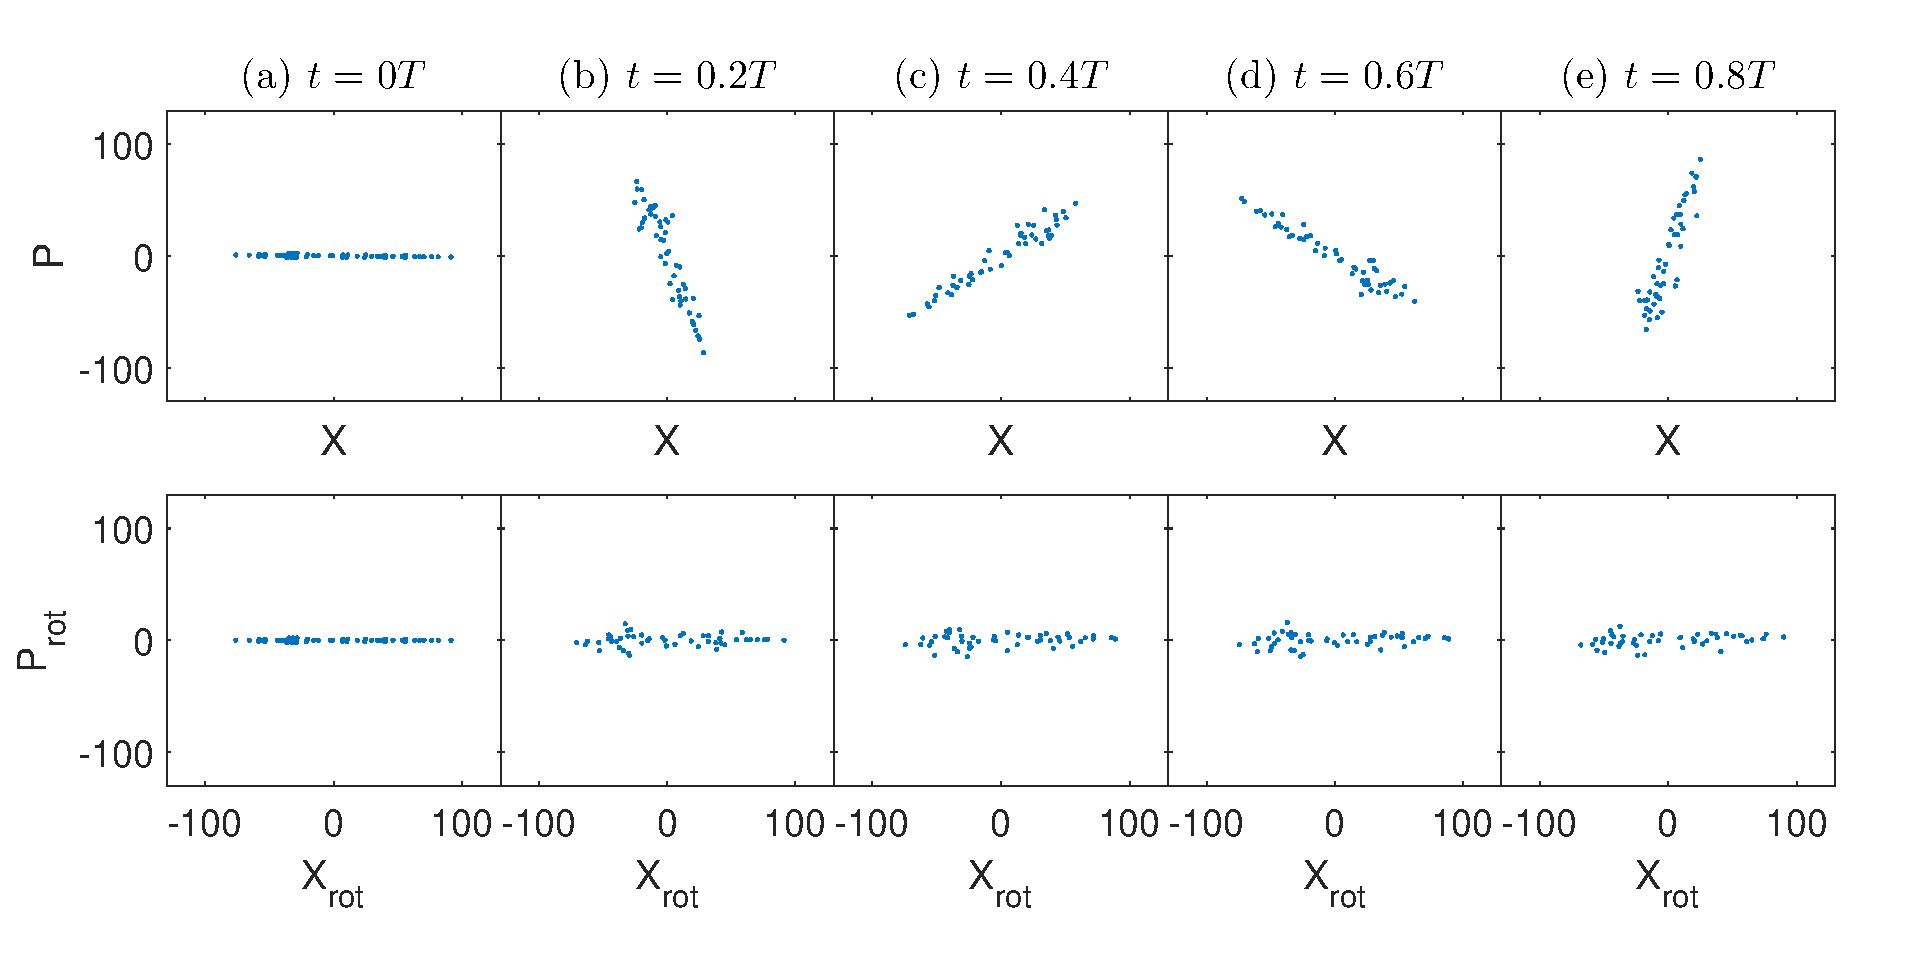
\includegraphics[width=0.9\textwidth]{ZhiyuPictures/stationary_and_rotating_frame_t=1-5_5T.eps}
%
\caption{Upper (lower) panels are snapshots of the cloud configuration in phase space in the
  stationary (rotating) frame, at instants within the first trap period.  Here $N=50$, $F_0=100$,
  and $E=50000$.  }
\label{fig:Breathingfrequency2_0}
\end{figure*}
%%%%% FIGURE %%%%% FIGURE %%%%% FIGURE %%%%% FIGURE %%%%% 


%%%%% FIGURE %%%%% FIGURE %%%%% FIGURE %%%%% FIGURE %%%%% 
\begin{figure*}
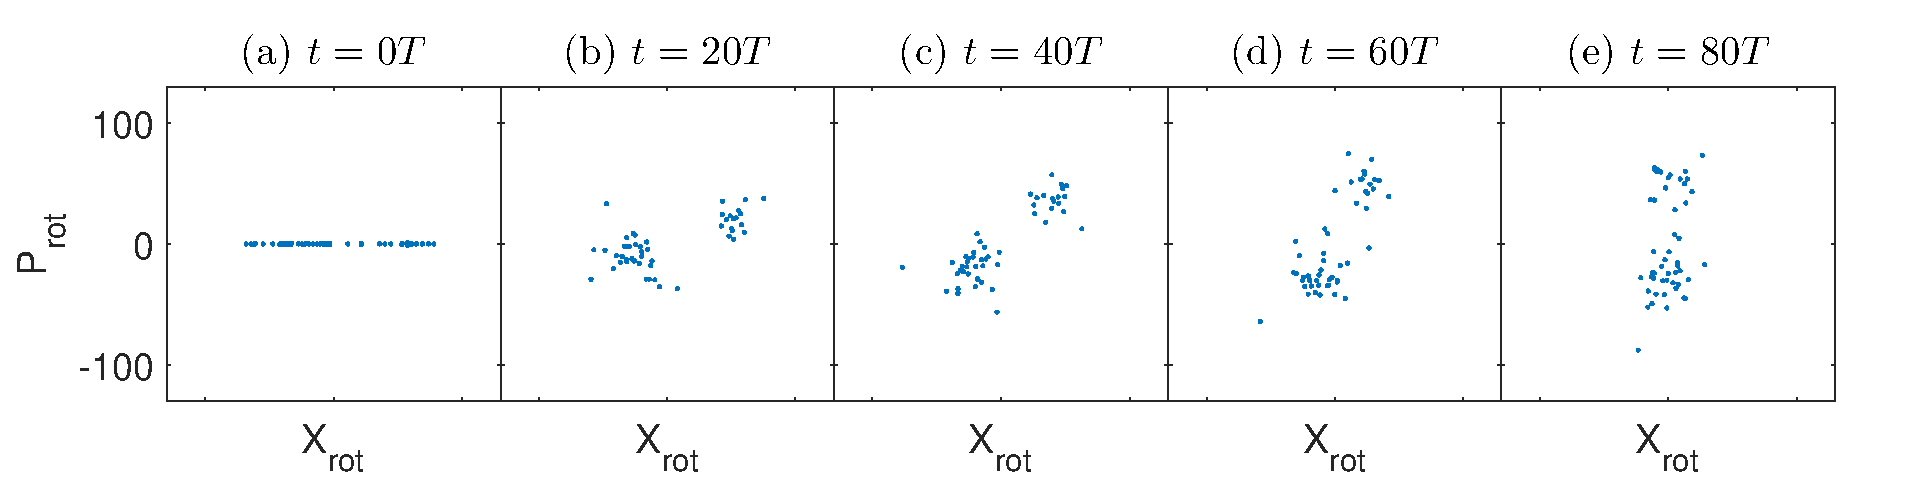
\includegraphics[width=0.9\textwidth]{ZhiyuPictures/rotating_frame_t=0-80T.eps}  
\caption{Phase space snapshots of the cloud dynamics viewed in the rotating frame, at longer
  timescales.  The broadening and rotation observed here are interaction effects: in the
  non-interacting gas the particles are stationary in this frame.}
\label{fig:Breathingfrequency2_1}
\end{figure*}
%%%%% FIGURE %%%%% FIGURE %%%%% FIGURE %%%%% FIGURE %%%%%

A useful way to visualize the state and evolution of the gas is to plot the position and momentum of
each particle, i.e., to plot the locations of the particles in the single-particle phase space.
This will be useful for visualizing both the breathing mode and relaxation. 

Figures \ref{fig:Breathingfrequency2_0} and \ref{fig:Breathingfrequency2_1} show such phase space
snapshots.  We generally start with particles distributed at random positions around the trap
center, initially with no velocity (zero momentum).  The initial state thus has the points lined up
along the $X$ axis.  In the absence of interactions, each particle would undergo simple harmonic
oscillation with period $T=2\pi/\omega_0 = 2\pi$.  The point corresponding to each particle executes
clockwise elliptical motion around the $X$-$P$ plane.  (In our units, the elliptical trajectory is
actually circular.)  This results in the initial line remaining a straight line and rotating
clockwise with exact period $T$.  The effect of the interaction is to smear out the line and spread
the points out toward a rotationally invariant distribution in the $X$-$P$ plane.  The top panel of
Figure \ref{fig:Breathingfrequency2_0} shows this during the first period and Figure
\ref{fig:Breathingfrequency2_1} shows this process over a much longer timescale.

Since the rotation of the initial line of points is simple to understand as a single-particle
(non-interacting) effect, we can focus on interaction effects by viewing the phase space in a
`rotating' frame.  The rotating frame is used in the lower panel of Figure
\ref{fig:Breathingfrequency2_0} and in Figure \ref{fig:Breathingfrequency2_1}.  In this picture, the
`real' $X$ and $P$ axes are rotating counter-clockwise.  This rotating frame picture may be regarded
as a classical version of the ``interaction picture'' of quantum dynamics.  This picture highlights
effects of interactions because the other effects are already encoded in the frame rotation.

In the absence of interactions, each point (each particle) is stationary in the rotating-frame
phase-space picture.  As seen in lower panel of Figure \ref{fig:Breathingfrequency2_0} and in Figure
\ref{fig:Breathingfrequency2_1}, interactions cause a gradual distortion of the line as well as some
degree of rotation.
%
The rotation that is visible in the already rotating $X_{\rm rot}$-$P_{\rm rot}$ frame is the
interaction-induced shift of the breathing frequency from the noninteracting value,
$\omega_B=2\omega_0$.  The distortion of the line toward an eventually rotationally invariant
distribution may be regarded as thermalization or ergodicity.  In the next sections we explore these
two interaction-induced effects.




\subsection{Numerical calculations}

We use the Verlet algorithm (molecular dynamics) to numerically simulate the cloud, using particle
numbers between 5 and 50.  Our force is simple, so that calculating the force at each step is
inexpensive, however, the theta function dependence of the force on particle positions requires the
use of fine timesteps at the beginning and end of each collision process.

The initial state is taken to have particles with zero velocity and random positions; hence the line
distribution in the phase space picture.  This has the advantage that the breathing motion is
prominently visible.  In addition, the question of long-time relaxation has the simple
interpretation of evolving from the line distribution to a circularly symmetric distribution.





%%%%% FIGURE %%%%% FIGURE %%%%% FIGURE %%%%% FIGURE %%%%% 
\begin{figure}[tbp]
\center
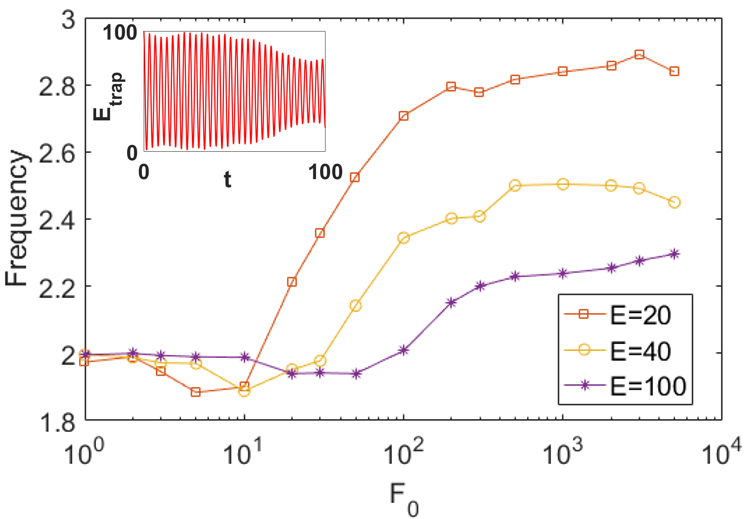
\includegraphics[scale=0.32]{ZhiyuPictures/freq_scanF_differentE_log_2_with_oscillation_demo.png}
\caption{Breathing mode frequency measured at different $E$ and $F_0$, for $N=5$ particles. Inset: a
  demonstration of the oscillation of $E_{trap}$, the total potential energy of particles in the
  trap, Since $E_{trap}\propto \sum_{is}{x_i^2}$, it manifests the oscillation behavior of the
  radius $R(t)$ as defined in Eq.~\ref{eq:def_of_R}.  The breathing frequency is obtained from the
  Fourier transform of $R(t)$.}
\label{fig:Breathingfrequency1}
\end{figure}
%%%%% FIGURE %%%%% FIGURE %%%%% FIGURE %%%%% FIGURE %%%%% 


\section{Breathing Frequency}\label{section:breathing frequency}


We are interested in the oscillations of the size $R(t)$ of the cloud.  It is convenient that our
finite-size simulations start with a line distribution in phase space.  If we started with a state
whose configuration in phase-space deviates only slightly from circular symmetry, the oscillating
amplitude would be too small to be distinguished from noise.

Without interaction, the breathing mode frequency is exactly 2.  This is visualized readily from the
top panel of \ref{fig:Breathingfrequency2_0}, where $R(t)$ is the extent of the distribution in the
horizontal ($X$) direction.  As the line rotates clockwise with frequency $\omega_0=1$, within each
period the line is twice horizontally aligned (maximum $R$) and twice vertically aligned (minimum
$R$), so that the frequency of $R(t)$ is $\omega_B=2$.  When there is interaction, the frequency
will get shifted: $\omega_B = 2+\delta$.  We measure the radius of the cloud $R(t)$ and get the
frequency spectrum of its oscillation behavior by Fourier transform. Then we take the peak frequency
near 2 as the breathing mode frequency.

The frequency measured in this way for different $E$ and $F_0$ is shown in the
Fig.\ref{fig:Breathingfrequency1}, plotted as a function of $F_0$.  The points each correspond to
breathing-mode dynamics following from a single initial state; there is no averaging.  The curves
therefore show some randomness.  However, two prominent features are clear from these curves.  At
large interactions, $F_0\gg E$, the breathing frequency is larger than $2$, and saturates around a
value which decreases with the system energy $E$.  At small interactions, the breathing frequency is
actually smaller than the non-interacting value $2$.   

Below, we will provide a detailed phase-space argument for these behaviors.  However, a simple
real-space picture explains both effects qualitatively as well.  For very large $F_0$, when the
interaction is `hard-core'-like, two particles exchange momentum immediately at a collision.  By
exchanging the labels of the particles during the collision, this can be interpreted as follows:
particle $A$ carrying momentum $P_A$ jumps by distance $\sigma$ to the right, while particle $B$
carries its momentum $P_B$ and jumps by distance $\sigma$ to the left.  In this manner, every
collision will save a particle some time, $\frac{\sigma}{v}$.  This translates into an increase of
the breathing frequency.  The speed $v$ per particle is on average $\sim\sqrt{E/N}$, and the number
of collision each particle experiences in one period of harmonic oscillation is $\sim N$; hence we
obtain $\delta\sim N^{\frac{3}{2}}E^{-\frac{1}{2}}$.  When $F_0$ is smaller, we can no longer think
of the particles as hard rods; the collisions now take finite time during which the speeds of the
particles are actually slowed down and then sped up again, as they either cross paths or bounce from
each other.  When $F_0$ is small enough, this approaching time will at some critical value of $F_0$
consume the time saved by the finite range of the interaction.  This explains why there is a
small-$F_0$ regime for which the shift $\delta$ is negative.  Figure \ref{fig:Breathingfrequency1}
shows that this critical value of $F_0$, where $\delta$ changes sign and $\omega_B$ crosses $2$,
increases with energy.


\subsection{Estimates using the rotating phase space}

Since we are interested in the deviation $\delta=\omega_B-2$ from the non-interacting breathing
frequency, it is useful to work in the rotating frame, in which a non-interacting cloud would be
stationary (non-rotating).  The rotation frequency of the cloud in this frame is then $\delta$.


%%%%% FIGURE %%%%% FIGURE %%%%% FIGURE %%%%% FIGURE %%%%% 
\begin{figure}[h
]
\subfigure[]{
\begin{minipage}[b]{0.4\textwidth}
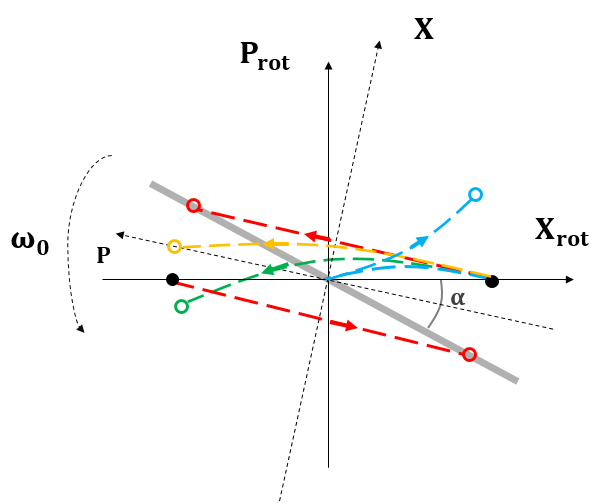
\includegraphics[width=1\textwidth]{ZhiyuPictures/bounce.png}
\end{minipage}
}
\subfigure[]{
\begin{minipage}[b]{0.4\textwidth}
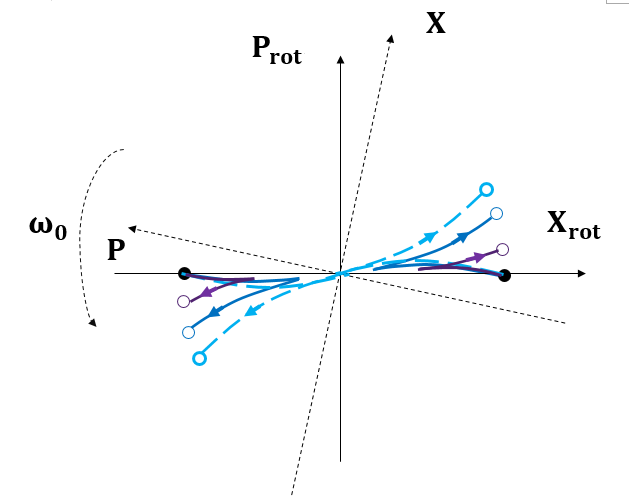
\includegraphics[width=1\textwidth]{ZhiyuPictures/pass.png}
\end{minipage}
}
\caption{Schematic diagrams of two-particle collision process in the $X_{\rm rot}$-$P_{\rm rot}$
  plane. \textbf{(a)}When $F_0$ is large, particles cannot pass each other.  Being subject to a
  constant repulsive force, their trajectories during collision are circular arcs.  For very strong
  interactions (red dashed line, straight), they exchange momenta instantaneously.  The yellow,
  green, and blue dashed curves are for successively weaker interactions.  \textbf{(b)} When $F_0$
  is small, particles pass each other, so that the force they feel is not continuous.  Their
  trajectory has a turning point. The dashed bright blue trajectory is identical with the one in
  (a), which is the critical situation between passing and bouncing. In that case, particles have
  zero relative velocity when they collide. }
\label{fig:Breathingfrequency3}
\end{figure}
%%%%% FIGURE %%%%% FIGURE %%%%% FIGURE %%%%% FIGURE %%%%% 



To analyze the rotation relative to the $X_{\rm rot}$-$P_{\rm rot}$ frame, we consider two-particle
collisions.  In Figure \ref{fig:Breathingfrequency3}(a), we show schematics of such a collision near
the trap center at strong interactions.  For very large $F_0$, the particles simply exchange momentum
when they are at distance $\sigma$ from each other; this process is shown in red as two straight
lines.  (The particles are initially at $X=\pm\frac{1}{2}\sigma$ and remain at these $X$ values,
but exchange their momenta.)   For smaller $F_0$, there is change of both position and momentum, as shown in yellow, green
and blue for successively weaker interactions. The blue line shows a case where $F_0$ is smaller
enough such that the particles can actually cross each other.

In Figure \ref{fig:Breathingfrequency3}(a) we show collisions for small $F_0$, so that the particles
pass each other.  The force changes direction discontinuously when the particles cross.  In the
$X_{\rm rot}$-$P_{\rm rot}$ plane, this is seen as a sharp turning point in the trajectory.

We now estimate $\delta$ at large $F_0$.  The relevant collision process is that shown by the red
lines in Figure \ref{fig:Breathingfrequency3}(a).  The two particles, which are initially on the
$X_{\rm rot}$ axis, are moved to two other points, on the thick gray line, which deviates a small
angle $\alpha$ away from original configuration.  In every period of the harmonic oscillation, each
particle meets each of the other particles twice.  Half of these collisions (about $N$ collisions)
are between particles with large difference in momentum, which is the process shown in
Fig.\ref{fig:Breathingfrequency3}.  (As for the remaining half of the collisions, colliding
particles have smaller difference in their momenta.  In this estimate we ignore the effects of these
collisions, as they clearly contribute far less to the rotation of the particle distribution.)

The precession angle is $\alpha\sim \sigma/P$.  In our rescaled units, the typical momenta of
interacting partilces is of the order $R$.  (In phase space $R$ can be interpreted either as the
extent in real space when the velocities are small, or as the extent in momentum space when the
particles approach $x=0$, i.e. when the distribution is along the $P$ direction.)  Thus, we can
estimate $\alpha\sim \sigma/R$, i.e., $\alpha\sim 1/R$, since our unit of length is $\sigma$.  This
is the rotation per unit collision.  Since there are $\sim N$ collistions per period $T=2\pi$, we
have the estimate for the interaction-induced rotation per unit time as
\begin{equation}
\delta ~=~ 2 \frac{N}{2\pi} \frac{1}{R} ~=~  \frac{1}{\pi}  N^{3/2}E^{-1/2}
\label{eq:breathingfrequency1}
\end{equation}
The factor $2$ accounts for the fact that each rotation of the elongated cloud in phase space
corresponds to two breathing mode periods.  In the last step we have used the estimate $E\sim
NR^2$. 

The effect of interaction on breathing frequency is more complicated at smaller $F_0$.  As we have
seen in Figure \ref{fig:Breathingfrequency1}, the effect of a small $F_0$ is to \emph{decrease} the
breathing frequency from its non-interacting value $\omega_B=2$.  This can also be understood using
phase-space pictures of collision processes.  For $F_0$ is not very big, the finite interaction time
needs to be taken into consideration.  During this time, the motion of each particle in phase-space
is moving exactly along the direction of the real $P$ axis at the rate $F_0/m$. Since the real $P$
axis is rotating counter-clockwise, the particle will follow a circular trajectory, e.g., following
the orange or green dashed lines in Fig.~\ref{fig:Breathingfrequency3}(a).  The angle $\alpha$ that
we used above to estimate $\delta$ thus decreases with the increase of interaction time; it is
smaller for the yellow line and even opposite for the green line.  This explains the negative
contribution of interaction to $\delta$, for small enough values of $F_0$.  At even smaller values
of $F_0$, shown in Fig.~\ref{fig:Breathingfrequency3})(b), the particles cross each other.  The
resulting final values are such that the line joining the post-interaction locations of the two
particles has negative $\alpha$, i.e., is tilted clockwise with respect to the $X_{\rm rot}$ axis,
meaning a negative contribution to the breathing frequency.

We can also estimate the critical value of $F_0$ for a given energy (or alternatively the critical
value of $E$ for a given $F_0$) between positive and negative contributions to the breathing
frequency.  Since the $P$ axis rotates with frequency $\omega_0=1$ in the $X_{\rm rot}$-$P_{\rm
  rot}$ plane, the post-collistion position of the particle in the $X_{\rm rot}$-$P_{\rm rot}$ plane
makes angle $\omega_0\tau$ with the red line in Figure \ref{fig:Breathingfrequency3}(a).  Here
$\tau$ is the time over which the interaction acts.  The crossover between positive and negative
$\delta$ is found by comparing this angle to $\alpha$:
\begin{equation}
\omega_0 \tau=\alpha
\end{equation}
The time $\tau$ is approximately the time it takes for the momentum to change sign due to a constant
force $F_0$, since the momentum is $\sim R$, this means $\tau\sim R/F_0$.  Using our previous
estimate  $\alpha\sim \sigma/R$, together with $E\sim NR^2$, gives us the condition
\begin{equation}
  \frac{E}{N} \sim F_0
  \label{eq_freq_turning_condition}
\end{equation}
for the breathing frequency to cross the non-interacting value $\omega_B=2$.  This is roughly the
same criterion for whether two particles will bounce or cross each other in a typical collision.

The condition \eqref{eq_freq_turning_condition} is consistent with Figure
\ref{fig:Breathingfrequency1}, where we noted that the critical $F_0$ grows with increasing energy.


\subsection{Comparisons with numerical data}


%%%%% FIGURE %%%%% FIGURE %%%%% FIGURE %%%%% FIGURE %%%%% 
\begin{figure}[h]
\centering
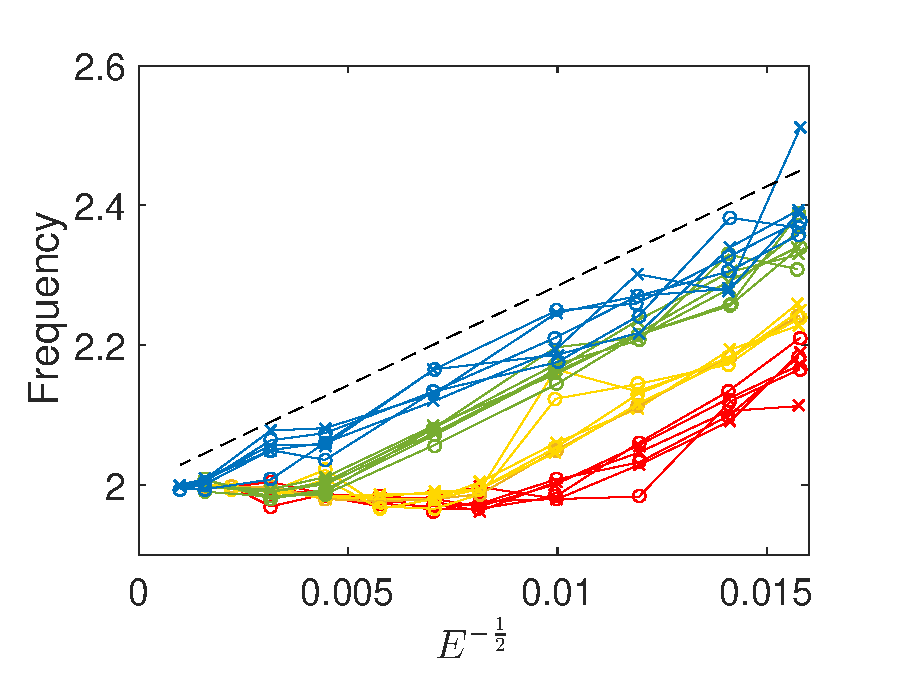
\includegraphics[scale=0.6]{ZhiyuPictures/freq_scanF_scanE_pre_Font18.eps}
\caption{Dependence of breathing frequency, calculated for $N=20$ particles, on energy.  Different
  colors represent different $F_0$ --- red for $F_0=2\times10^3$, yellow for $F_0=3\times10^3$,
  green for $F_0=1\times10^4$, and blue for $F_0=1\times10^5$.  Runs with three different initial
  states are shown in each case.  In each run, the frequency is measured both in the time window
  0-100 (labeled as crosses) and in the time window 900-1000 (labeled as circles). The black dashed
  line is the prediction of Eq.~\eqref{eq:breathingfrequency1}.}
\label{fig:Breathingfrequency4}
\end{figure}
%%%%% FIGURE %%%%% FIGURE %%%%% FIGURE %%%%% FIGURE %%%%% 


In Figure \ref{fig:Breathingfrequency4} we show a quantitative test of the main rotating-phase-space
prediction, Eq.~\eqref{eq:breathingfrequency1}.  For large $F_0$, the frequency indeed scales as
$E^{-1/2}$ and for $F_0=10^5$ is quite close to the actual numerical values prediction
\eqref{eq:breathingfrequency1}.  Even for smaller $F_0$, at small enough energies (larger $E^{-1/2}$
values) the breathing mode becomes proportional to  $E^{-1/2}$. 

One might ask whether the breathing frequency predictions are also valid at late times, after the
system has `relaxed' from the initial line distribution in phase space to a more spread-out cloud,
as we have seen in Figure \ref{fig:Breathingfrequency2_1}.  In \ref{fig:Breathingfrequency4} we show
the breathing frequency calculated from $R(t)$ oscillations in the first 100 time units, and also
the frequency from data in a later time window. The frequencies appear to be overall stable and dependent
primarily on $F_0$ and $E$.  




\section{Thermalization}\label{section:Thermalization}


For any nonzero interaction, the system is expected to be ergodic for $N>2$.  Once there are many
particles, one expects thermalization in the long-time limit.  From the few-particle perspective,
several interesting questions pose themselves.  First, although we expect ergodicity, the question
of how long it takes to thermalize is an open question for small $N$. We treat below a
coarse-grained version of this question: namely, we ask whether particles show ergodic behavior
within reasonable timescales chosen to be (somewhat arbitrarily) in the timestep range of
$10^3$--$10^4$.  Another question is the connection between thermalization, as defined by the
appearance of a Boltzmann distribution and other intuitive characteristics of ergodic behavior such
as whether the single-particle phase space is isotropically occupied.  We find cases where one
aspect is seen while the other is not.  

In the subsections below, we first ***  then **** 






\subsection{Few-particle considerations}

Since we are interested in thermalization within finite timescales, it is useful to consider
mechanisms which hinder relaxation or thermalization.  We begin with considerations of few-particle
motion.  Since ergodicity and relaxation are generally expected to be more robust and efficient with
larger particle numbers, consideration of small particle numbers will highlight effects which slow
down relaxation.



%%%%% FIGURE %%%%% FIGURE %%%%% FIGURE %%%%% FIGURE %%%%% 
\begin{figure}[tbph]
\centering
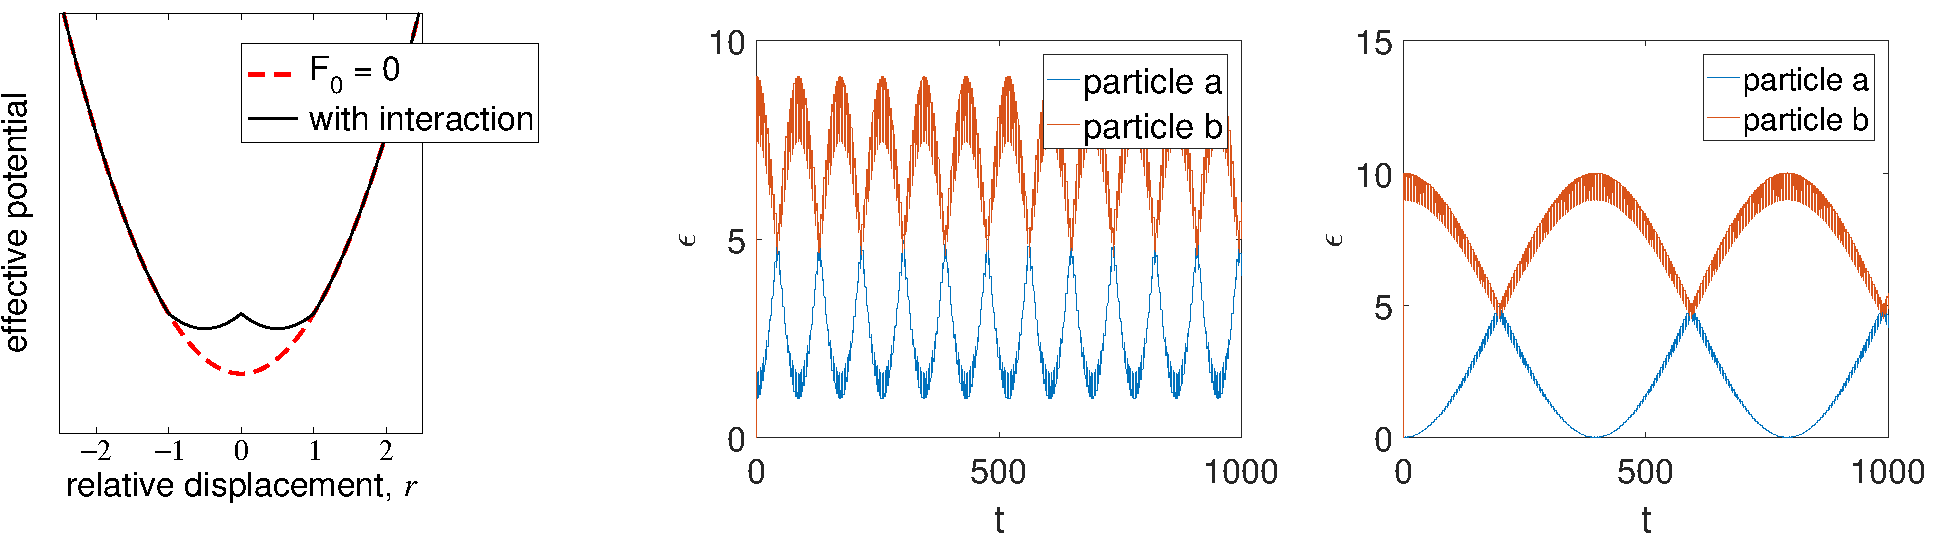
\includegraphics[width=0.9\textwidth]{ZhiyuPictures/two_particles_a_01.pdf}
\caption{Left: Effective potential for two-particle system.  Center and right: beats at internal
  energy $E_i=2$ and $E_i=5$.  The curves show the individual energies of the two particles.  Here
  $F_0=1$. In this case, the larger the $E_i$, the lower the beat frequency. }
\label{fig:thermalization2}
\end{figure}
%%%%% FIGURE %%%%% FIGURE %%%%% FIGURE %%%%% FIGURE %%%%% 


\subsubsection{Two particles}

We consider the two-particle motion in their center of mass frame.  The center of mass itself
executes simple harmonic oscillation.  In the absence of interactions ($F_0=0$), the effective
potential within the center of mass frame is itself parabolic, with the same frequency.  So their
relative motion is also a harmonic oscillation, with the same frequency $\omega_0$.

With interactions, a term $F_0(1-|r|)\theta(1-|r|)$ is added, where $r$ is the relative
displacement; as shown in Figure \ref{fig:thermalization2}.  Now, the relative motion is no longer
harmonic; one could regard the resulting motion has having a slightly different frequency, or a
collection of frequencies whose center is shifted slightly from $\omega_0$.  Since the
center-of-mass motion is still of frequency $\omega_0$, we have a superposition of slightly
different frequencies, resulting in beating dynamics.  This is clearly seen in the time evolution of
individual energies shown in Figure \ref{fig:thermalization2}.  The two panels correspond to
different internal energy $E_i$ (defined as the total energy minus the center-of-mass energy).  For
larger $E_i$, the distortion of the effective potential (at constant $F_0$) plays a smaller role in
shifting the effective frequency of relative motion; hence the beat frequency is smaller.  

This illustrates a simple mechanism hindering the redistribution of energy between particles, which
is necessary for thermalization or relaxation.  As seen in the example dynamics shown, the
difference in energy between the two particles is sustained over time.  Of course thermalization is
not expected anyway in a two-particle system, but we will see below how this basic effect continues
to play a role for larger $N$.

-------



%% \begin{figure}[h]
%% \subfigure[$E_i=2$]{
%% \begin{minipage}[b]{0.22\textwidth}
%% 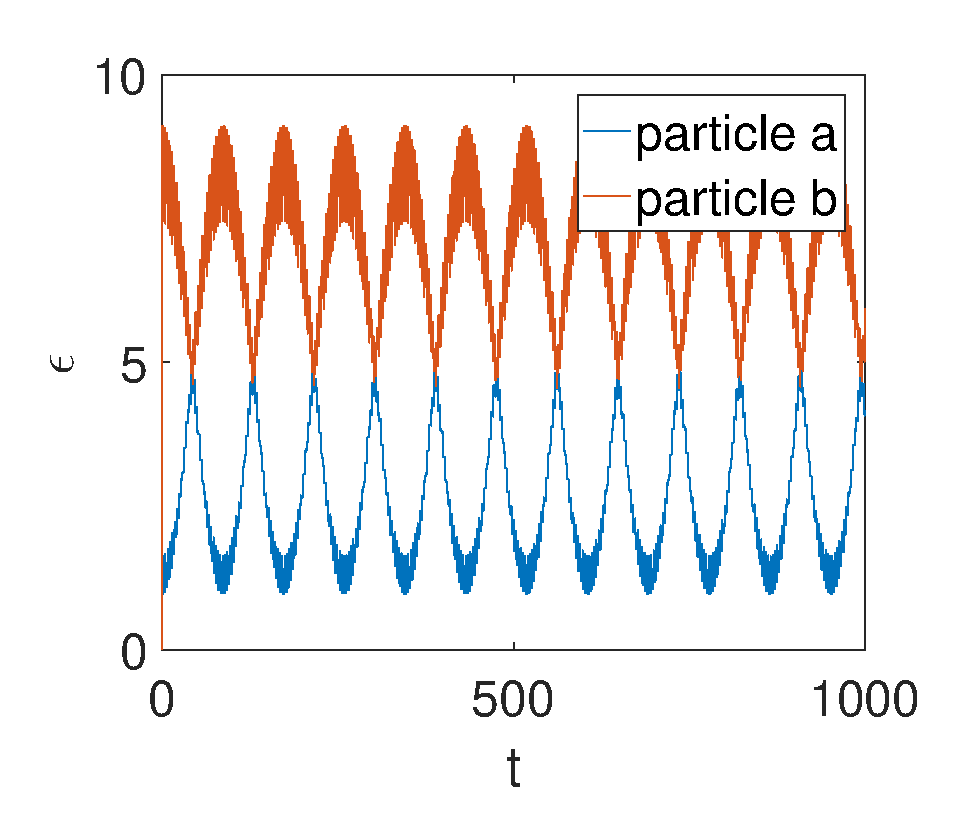
\includegraphics[width=1\textwidth]{ZhiyuPictures/10_23_N=2_F0=1_Er=2_single_particle_energy_600_500_Font24.eps} 
%% %\includegraphics[scale=0.2]{ZhiyuPictures/twoparticle_Er=2_phasespace.eps}
%% \end{minipage}
%% }
%% \subfigure[$E_i=3$]{
%% \begin{minipage}[b]{0.22\textwidth}
%% 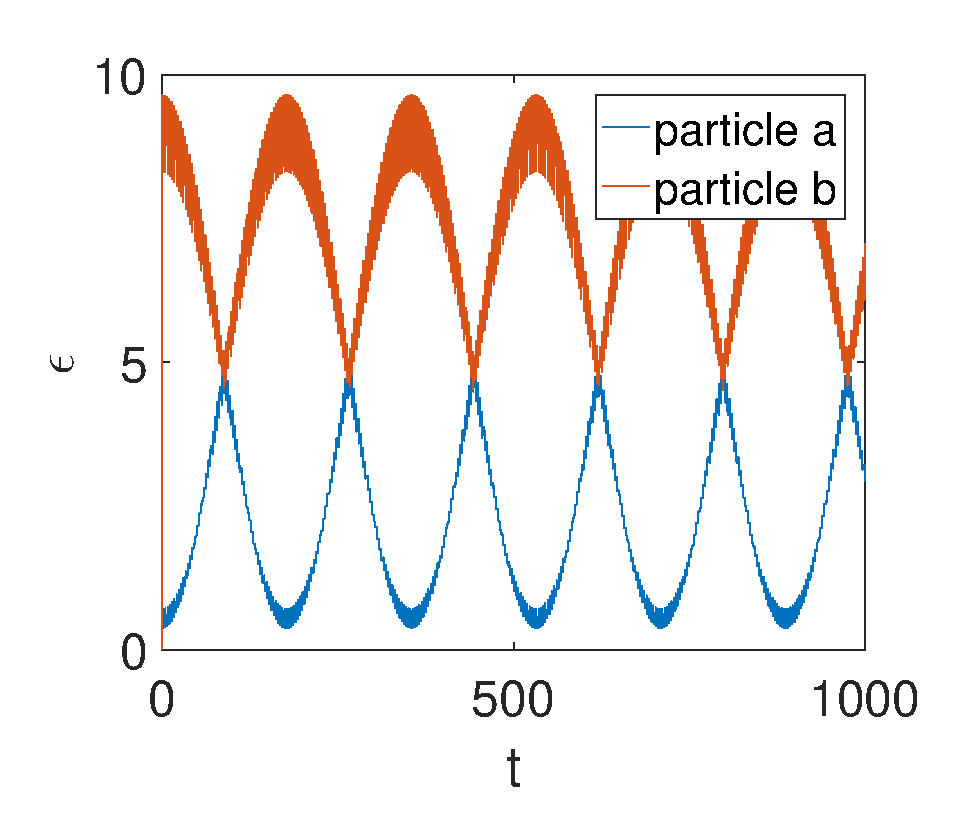
\includegraphics[width=1\textwidth]{ZhiyuPictures/10_23_N=2_F0=1_Er=3_single_particle_energy_600_500_Font24.eps} 
%% %\includegraphics[scale=0.2]{ZhiyuPictures/twoparticle_Er=3_phasespace.eps}
%% \end{minipage}
%% }
%% \subfigure[$E_i=5$]{
%% \begin{minipage}[b]{0.22\textwidth}
%% 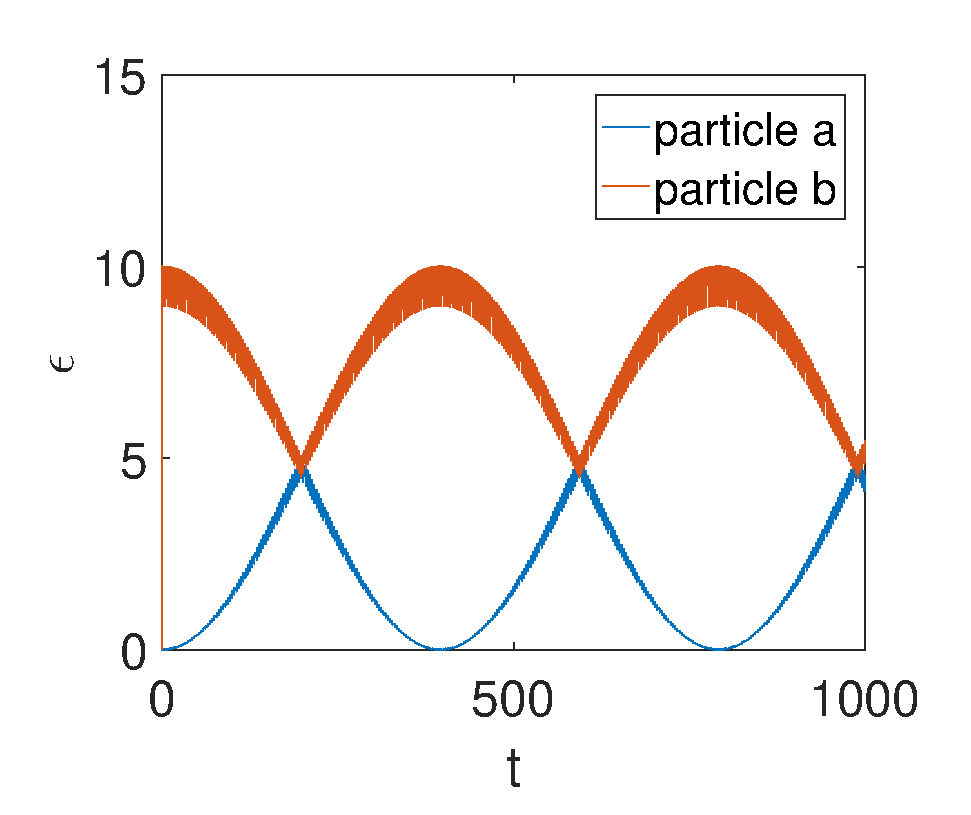
\includegraphics[width=1\textwidth]{ZhiyuPictures/10_23_N=2_F0=1_Er=5_single_particle_energy_600_500_Font24.eps} 
%% %\includegraphics[scale=0.2]{ZhiyuPictures/twoparticle_Er=5_phasespace.eps}
%% \end{minipage}
%% }
%% \subfigure[$E_i=10$]{
%% \begin{minipage}[b]{0.22\textwidth}
%% 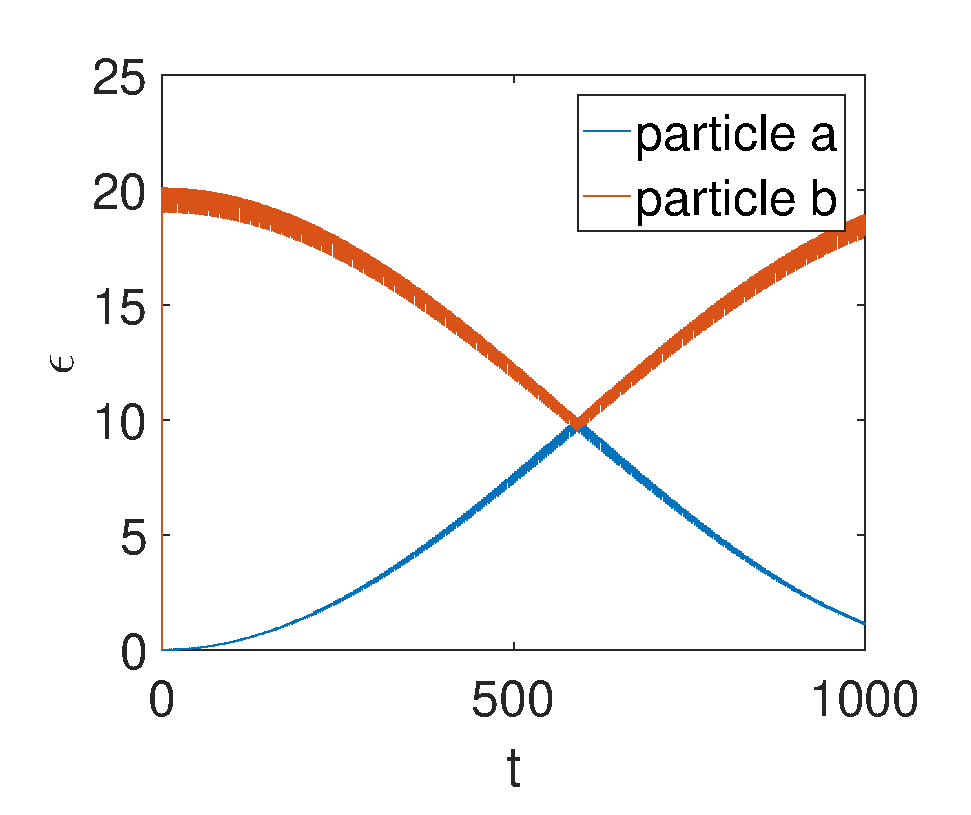
\includegraphics[width=1\textwidth]{ZhiyuPictures/10_23_N=2_F0=1_Er=10_single_particle_energy_600_500_Font24.eps} 
%% %\includegraphics[scale=0.2]{ZhiyuPictures/twoparticle_Er=10_phasespace.eps}
%% \end{minipage}
%% }

%% \caption{the dependence of beat frequency on internal energy. The diagram is the energy of two
%%   particles. Here, $F_0$ is set to be 1. In this case, the larger the $E_i$, the lower the beat
%%   frequency. \label{fig:thermalization1}}
%% %Actually in very low energy, we can retrieve a beat, but that is for different reason -- it is a
%% %beat between $\omega_0$ and $\frac{\omega_0}{2}+\delta $
%% %
%% \end{figure}




\subsubsection{More particles}

Now let's consider the three-particle case. For two particle, the motion is non-chaotic. On the other hand, intuitively, we will say that three-body motion is chaotic so that the system could be ``thermalized" soon. However, in some cases, the time scale of thermalizing could still be very long. Suppose two of them, say, A and B, has small internal energy, which means their distance and relative velocity are both small. Meanwhile, suppose particle C has some energy quite different from A \& B. In this case, A \& B will often be in the interaction, while C will pass both of them at a high speed in each period. How will energy transfer between C and the two-particle system A and B? Since the relative velocity of C and the two-particle system is usually large, C will pass A-B pair in a short time $\tau\sim\frac{\sigma}{R}$ ($\tau\ll\frac{2\pi}{\omega}$). C gives A a push when approaching it, and then push A back when leaving.  As has been discussed in the two-particle case, this process is equivalent to giving A a very small velocity ($\sim O(\frac{\sigma}{R})$) in the background of a trap. Since both the position and velocity of A and B are close($|x_A-x_B|\sim\sigma$), the velocity increase of A \& B are almost the same (difference$\sim O(\frac{\sigma^2}{R^2})$). In this manner, the passing of particle C only kicks the center of mass of the A-B pair slightly, leaving the internal motion of the pair unaffected. In another word, the existence of C will not have significant effect on the energy transfer between A and B, but only ``dance" with their center of mass. The physics of the ``dance" is similar to the dance between two particle. As is shown in Fig.\ref{fig:thermalization4}, the particles with energy close to each other tends to form a pair with small internal energy and the pair's internal energy transfer is relatively stable.


%%%%% FIGURE %%%%% FIGURE %%%%% FIGURE %%%%% FIGURE %%%%% 
\begin{figure}
\centering
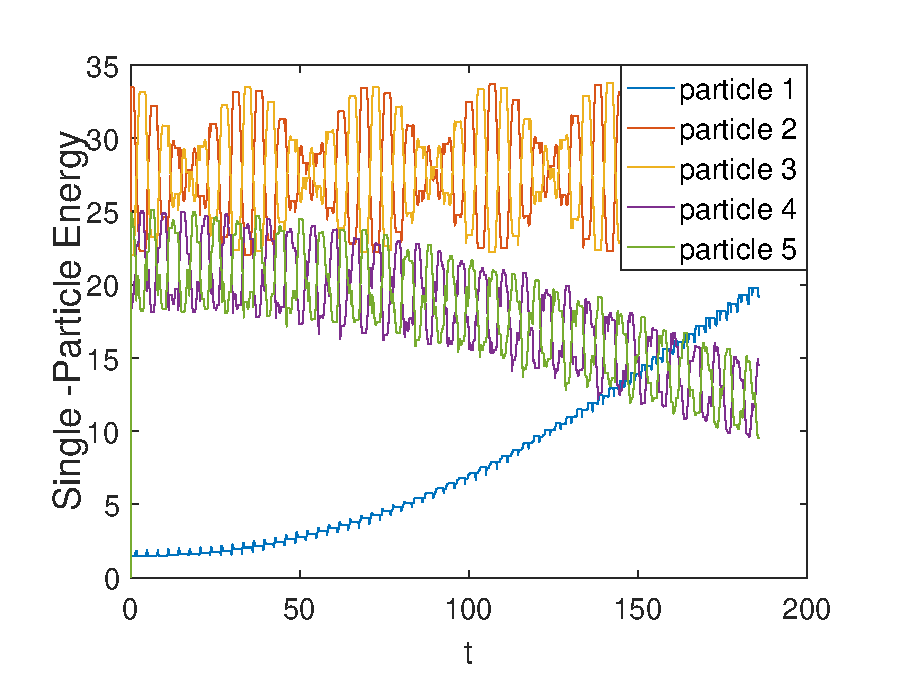
\includegraphics[scale=0.5]{ZhiyuPictures/pair1_pre.eps}
\caption{Time evolution of single-particle energy}
\label{fig:thermalization4}
\end{figure}
%%%%% FIGURE %%%%% FIGURE %%%%% FIGURE %%%%% FIGURE %%%%% 


The argument above still holds in many-particle case. Once we start from some configuration where n particles have a set of close energy levels $\left\lbrace E_n\right\rbrace $ and another m particles have another set of energy levels close to each other $\left\lbrace E_m\right\rbrace $, and $\left\lbrace E_n\right\rbrace $ is quite different from $\left\lbrace E_n\right\rbrace $, we will find these two systems oscillating on the energy level diagram at low frequency. 
The discussion above gives us some pictures about the non-ergodic state. For these state, life time is rather long so that once the system reach such configuration (or certain energy distribution), it will take a long time(more than $10^4$ periods for N=5 case) to decay. 

\subsection{Thermalization condition}
The main obstruct to get an thermalized state is the low frequency beat mentioned before. As a result, to achieve ergodic state, we have to avoid such low frequency oscillation. According to our discussion before, the solution is to make internal energy of each two-particle pair not ``too large". Though it is impossible to express the internal energy of every pair in terms of the total energy $E$, we can estimate it by the average energy, which is $\frac{E}{N}$. At least they are of the same order. The thermalization condition could be given by:
\begin{equation}
F_0\sigma\sim\frac{E}{N}
\label{eq:thermalizatiton condition}
\end{equation}



%%%%% FIGURE %%%%% FIGURE %%%%% FIGURE %%%%% FIGURE %%%%% 
\begin{figure}[h]
\centering
%\includegraphics[scale=0.2]{ZhiyuPictures/distribution1_scanF0_E=100_3.eps}
%\caption{Distribution scan $F_0$, $E=100$, $N=5$, $\sigma=1$ {\color{red}{Run again!}} }
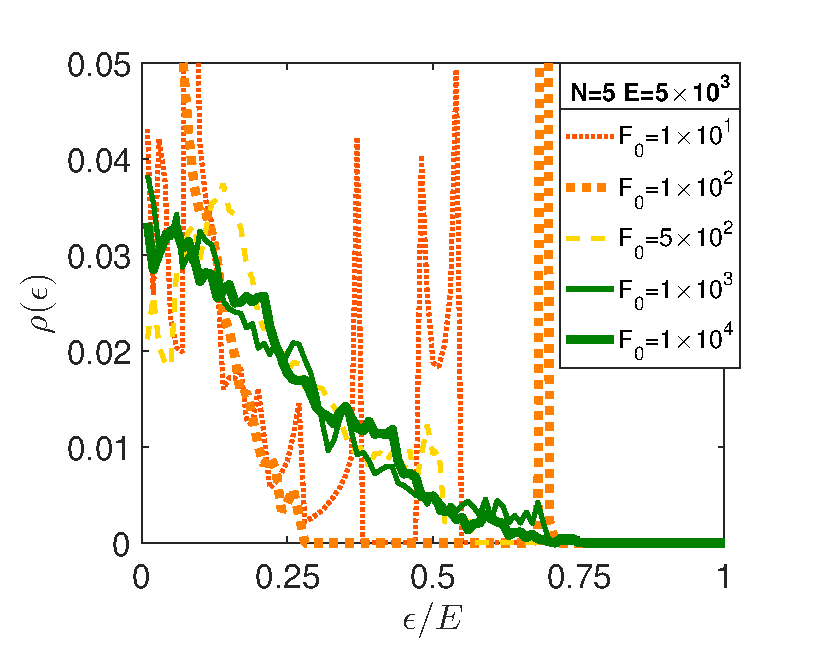
\includegraphics[width=0.32\textwidth]{ZhiyuPictures/N=5_energydistribution_500_400_Font16.eps} 
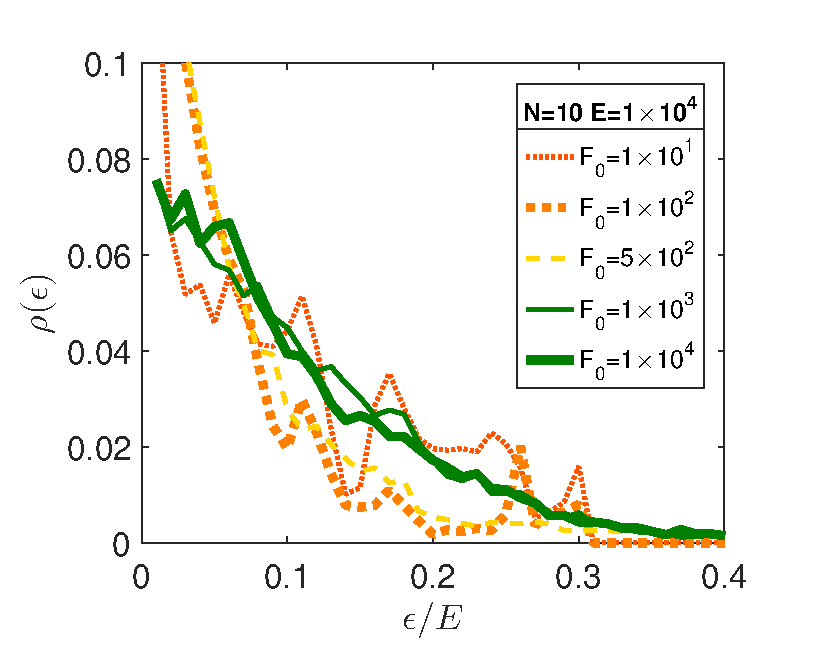
\includegraphics[width=0.32\textwidth]{ZhiyuPictures/N=10_energydistribution_500_400_Font16.eps}
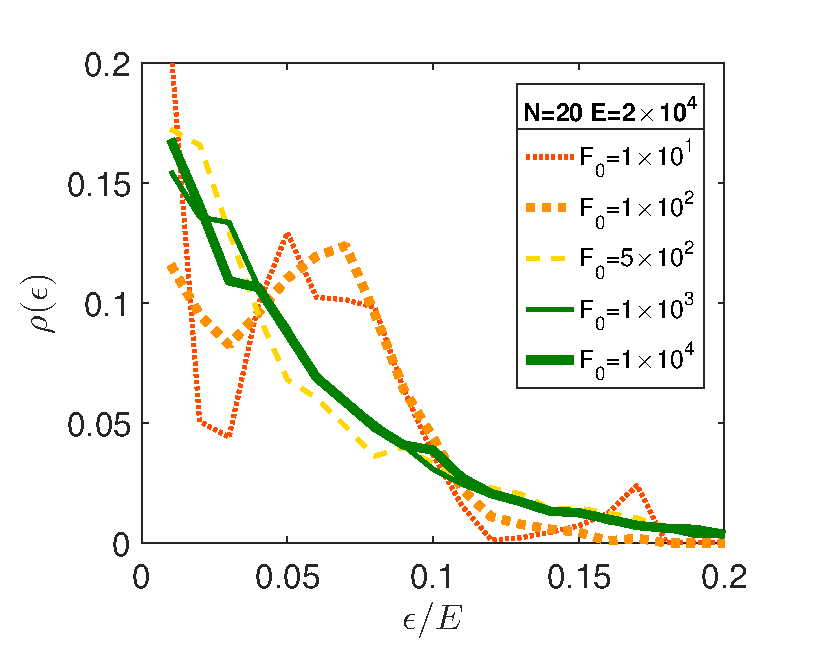
\includegraphics[width=0.32\textwidth]{ZhiyuPictures/N=20_energydistribution_500_400_Font16.eps}
\caption{the energy distribution measured in $\sim 10000$ time units, as will be verified later, Green curves corresponds to Boltzmann distribution; Red curves are obviously non-Boltzmann, while the yellow ones are intermediate case, represent ``thermalization threshold". In three figures for different N, we choose E/N identical (=1000), and thermalization is reached at $F_0=500\sim1000$, which is consistent with our prediction in Eq.\ref{eq:thermalizatiton condition}}
\label{fig:thermalization5}
\end{figure}
%%%%% FIGURE %%%%% FIGURE %%%%% FIGURE %%%%% FIGURE %%%%% 


%\begin{figure}
%\subfigure[N=10, $F_0=200$]{
%\begin{minipage}[b]{0.4\linewidth}
%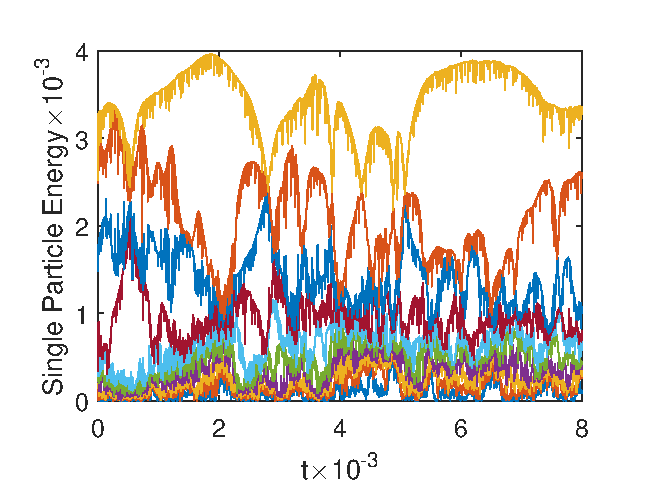
\includegraphics[width=1\textwidth]{ZhiyuPictures/N=10_single_particle_energy_F0=200_Font12_s.eps} 
%\label{fig:thermalization6}
%\end{minipage}
%}

%\subfigure[N=10, $F_0=1000$]{
%\begin{minipage}[b]{0.4\linewidth}
%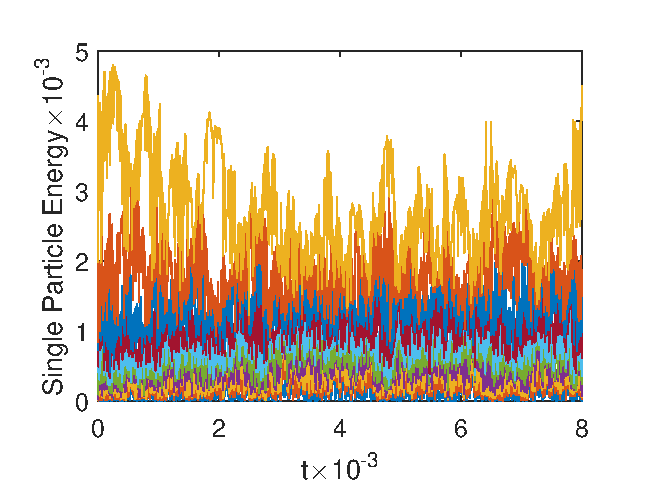
\includegraphics[width=1\textwidth]{ZhiyuPictures/N=10_single_particle_energy_F0=1000_Font12_s.eps} 
%\label{fig:thermalization7}
%\end{minipage}
%}

%\end{figure}


%%%%% FIGURE %%%%% FIGURE %%%%% FIGURE %%%%% FIGURE %%%%% 
\begin{figure}[h]
\subfigure[N=10, $F_0=200$]{
\begin{minipage}[b]{0.4\linewidth}
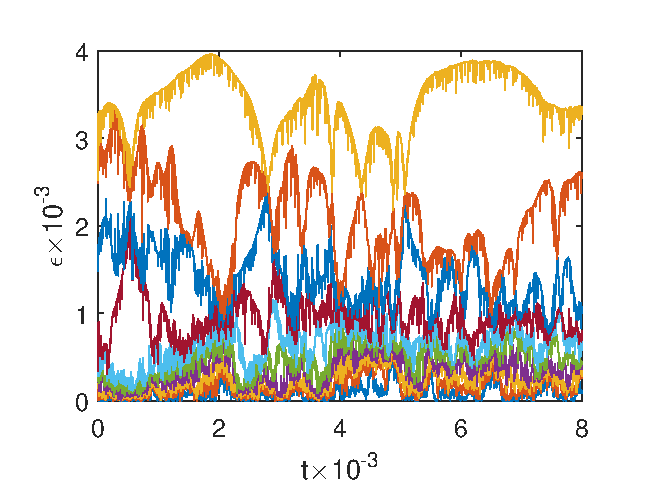
\includegraphics[width=1\textwidth]{ZhiyuPictures/N=10_single_particle_energy_F0=200_s_400_300_Font12.eps}
\label{fig:thermalization6}
\end{minipage}
}
\subfigure[N=10, $F_0=1000$]{
\begin{minipage}[b]{0.4\linewidth}
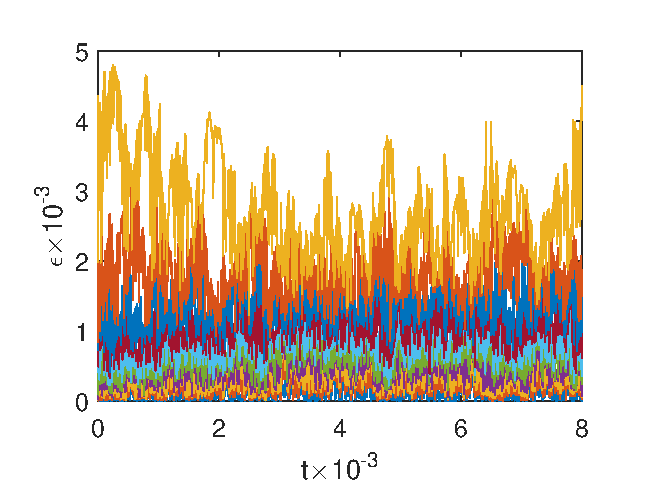
\includegraphics[width=1\textwidth]{ZhiyuPictures/N=10_single_particle_energy_F0=1000_s_400_300_Font12.eps} 
\label{fig:thermalization7}
\end{minipage}
}
\caption{Time evolution of the particles' energy $\epsilon$}
\end{figure}
%%%%% FIGURE %%%%% FIGURE %%%%% FIGURE %%%%% FIGURE %%%%% 


As is shown in Fig.\ref{fig:thermalization5} above, the critical point for reaching ``Boltzmann-like" distribution (later we will verify that it is Boltzmann distribution) is $F_0=500\sim1000$ (we always set $\sigma=1$), while the average energy $\sim 1000$, as we expected, they are of the same order. As a supplementary proof of our argument, Fig.\ref{fig:thermalization6} and Fig.\ref{fig:thermalization7} show the great difference of single-particle energy between two examples of below and above the thermalization threshold ($F_0=200$ $\&$ $F_0=1000$ for $N=10, E=10000$): in the former one there is always some particle maintained at high excitation, while in the latter the system probably goes to ergodic. To date, we have verified that the threshold of thermalization, which is $\frac{NF_0\sigma}{E}\sim1 $ , and corresponding feature of their energy distribution in two side of the threshold.

One may think that this condition only means that the energy transfer in every collision is much smaller than the energy interval. But this is not the whole story. The essential difference between these two regime lies in whether the energy transfer in every collision is correlated: In thermalizable regime, the energy transfer in every collision is much smaller than the energy interval, which definitely slows down the energy transfer. What is more, because of this, the particles is less interferred by other particles so that two-particle analysis survives. It means that for a particle pair, the energy transferred in this collision is correlated with the one in the next time. In this manner, each particle in the pair will pick up some energy in several collisions, and then return it back to its partner -- which is just what the low frequency beat effect tells us. Thus the particles energy is localized in certain value. On the contrary, if we go to non-thermalizable regime, the energy transfer is so fast that for each particle don't remember their partners. As a result, the energy transferred in every collision between two particles are no longer correlated so that our two-particle analysis breaks down. Instead, the energy transfer is completely random, with a non-zero amplitude. On the single-particle energy diagram, what we expected to see is a ``one dimensional random walk" ,so energy levels quickly spread around the diagram.

To sum up, the thermalization threshold not only tells us whether the amplitude of energy transfer in every collision is small enough compared to particles' energy, but also shows whether the ``correlation time" of particle pair is much longer than the characteristic time of the system (the oscillation period).  


\subsection{Verifying Boltzmann distribution}
Thermalization could have different definition. In our system, the ``thermalization" we want to find means ``losing all the memory of initial state". One of the most important information of initial state is energy distribution. 
 
For an isothermal system, the energy distribution of the whole system follows the Boltzmann distribution in equilibrium state. However, there is not any obvious conclusion about the distribution for an isolated system where the total energy is conserved. But intuitively, one will expect that if we measure the energy of a subsystem, e.g. one particle, then we will get a Boltzmann distribution because the rest part of the system can be considered as a bath for this particle. The temperature of this isolated system is defined according to $Nk_BT=E$. It is evident that this argument only hold when the energy of the single particle is not too big --- if one particle take up 50\% of the total energy, the rest could no longer be thought of as a good bath.

In the first picture below, we verify this argument by measuring the energy distribution of every particle at N=10 for different F0 at E=1000 (parameters here satisfy thermalizing condition). In the other two, we tested different N.


%\begin{figure*}
%%\includegraphics[scale=0.5]{ZhiyuPictures/distribution_at_N=5_F0=10000_pre.eps}
%%\caption{Energy distribution, N=5, F0=10000}
%%\label{fig:thermalization8}
%\subfigure[N=10, $F_0=1\times10^4$]{
%\begin{minipage}[b]{0.1\textwidth}
%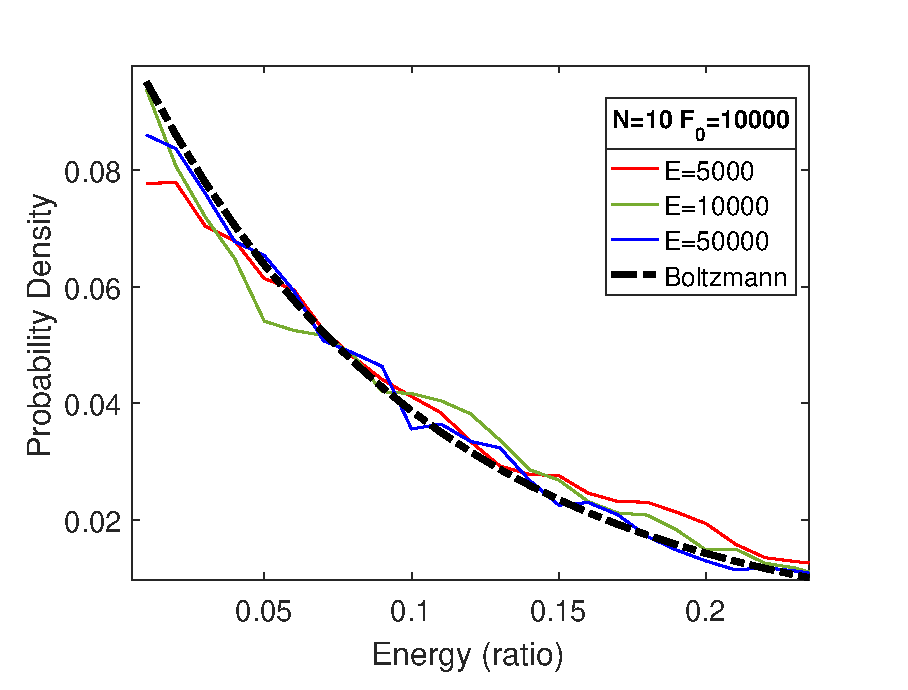
\includegraphics[scale=0.1]{ZhiyuPictures/boltzmann_N=10_F=10000_pre_rev.eps}
%\caption{Energy distribution, N=10, $F_0=1\times10^4$}
%\label{fig:thermalization9}
%\end{minipage}
%}

%\subfigure[N=20, $F_0=1\times10^4$]{
%\begin{minipage}[b]{0.1\textwidth}
%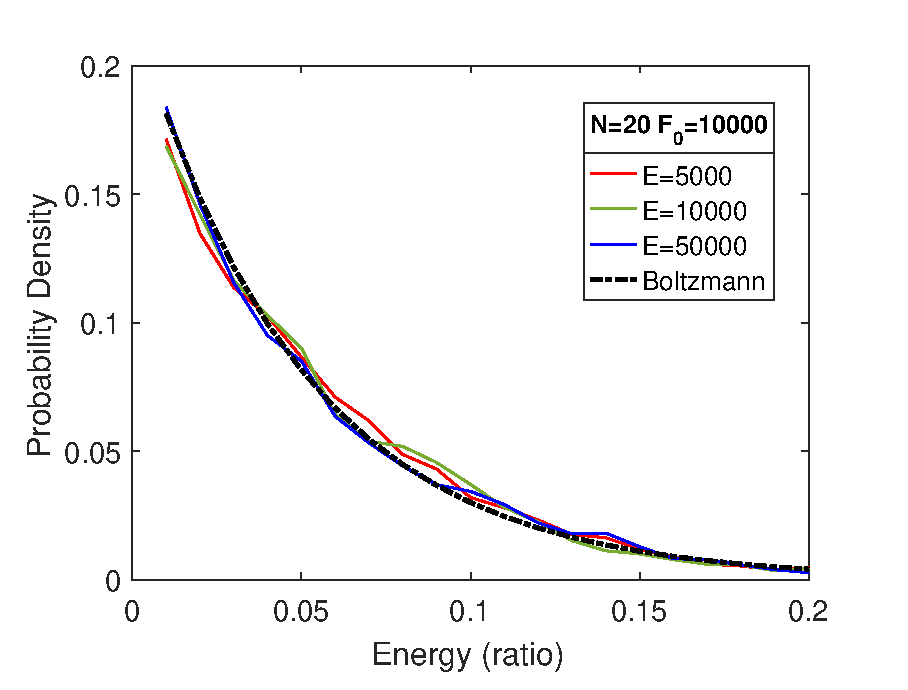
\includegraphics[scale=0.1]{ZhiyuPictures/boltzmann_N=20_F=10000_pre_rev.eps} 
%\caption{Energy distribution, N=20, $F_0=1\times10^4$}
%\label{fig:thermalization10}
%\end{minipage}
%}

%\end{figure*}

%%%%% FIGURE %%%%% FIGURE %%%%% FIGURE %%%%% FIGURE %%%%% 
\begin{figure}[h]
\subfigure[N=10, $F_0=1\times10^4$]{
\begin{minipage}[b]{0.4\linewidth}
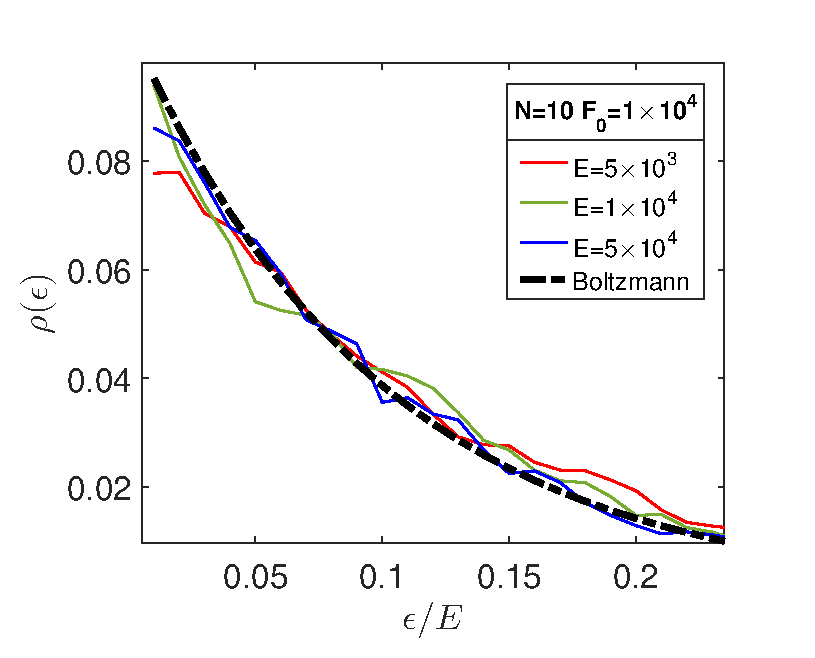
\includegraphics[width=1\textwidth]{ZhiyuPictures/boltzmann_N=10_F=10000_500_400_Font16.eps}
\label{fig:thermalization9}
%\caption{Energy distribution, N=10, $F_0=1\times10^4$}
\end{minipage}
}
\subfigure[N=20, $F_0=1\times10^4$]{
\begin{minipage}[b]{0.4\linewidth}
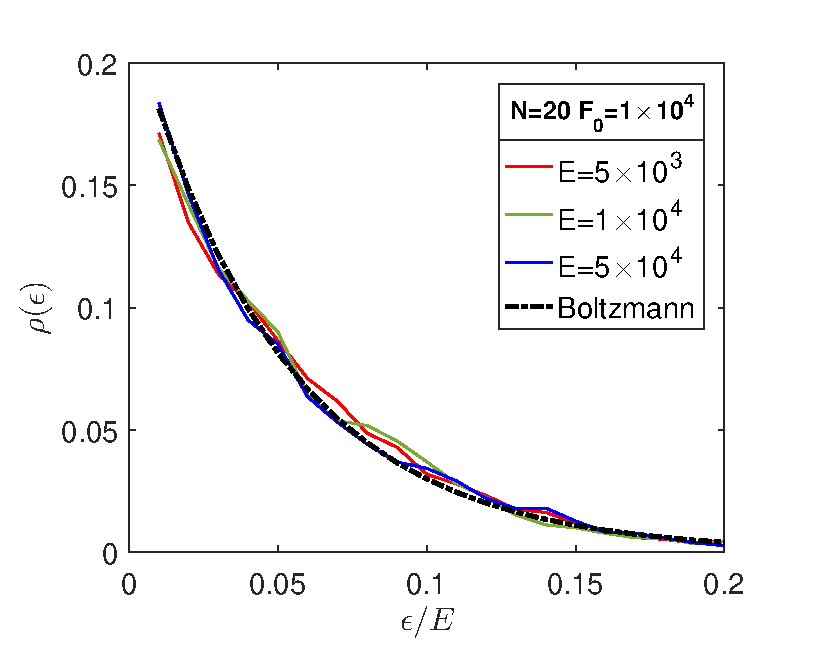
\includegraphics[width=1\textwidth]{ZhiyuPictures/boltzmann_N=20_F=10000_500_400_Font16.eps} 
\label{fig:thermalization10}
%\caption{Energy distribution, N=20, $F_0=1\times10^4$}
\end{minipage}
}
\caption{Fitting energy distribution $\rho(\epsilon)$ with Boltzmann distribution}
\end{figure}
%%%%% FIGURE %%%%% FIGURE %%%%% FIGURE %%%%% FIGURE %%%%% 

In Fig.\ref{fig:thermalization9} and Fig.\ref{fig:thermalization10}, the curve is slightly deviated
from the standard Boltzmann distribution, which is probably due to the contribution of density of
states (DOS). Possibility is proportional to Boltzmann exponential factor multiplied by density of
states. The reason why we did not take DOS into account previously lies in that the DOS is a
constant for simple harmonic oscillator. However, for simple harmonic oscillators with short range
interaction, the energy shell is deformed in the small region of $|x_i-x_j|<\sigma$ so that the DOS
is no longer a constant. The effect of interaction is conspicuous in low energy part: when
interaction is weak, particles prefer to stay near zero energy according to Boltzmann distribution,
but when interaction grows, they are no longer allowed to accumulate near zero energy, in another
word DOS at low energy decreases with the increase of interaction. Therefore, counts at the low
energy part of Fig.\ref{fig:thermalization9} and \ref{fig:thermalization10} is always a little bit
lower than the Boltzmann prediction. But since $\sigma<<R$, we can think of interaction as a small
modification, so the overall tendency still fits well.

\subsection{Lyapunov Exponents}
The Lyapunov Exponents is a good tool to quantify the time scale of ``thermalization". Lyapunov Exponents(LE) describes how fast one orbit diverge from its nearby orbits in $\Gamma$-space. But for high dimensional system, LE is a spectrum that manifest the instability of the trajectory along each direction. The largest Lyapunov exponents (LLE) reflects the shortest time scale that system lose its memory. Each point along one trajectory in $\Gamma$-space could have different LLE value, but the distribution of LLE is dependent on macroscopic parameters. As is shown in Fig.\ref{fig:LLEdistribution1}, we measured the LLEs along our trajectory and plot its distribution as a function of total energy.

\begin{figure}[h]
\centering
%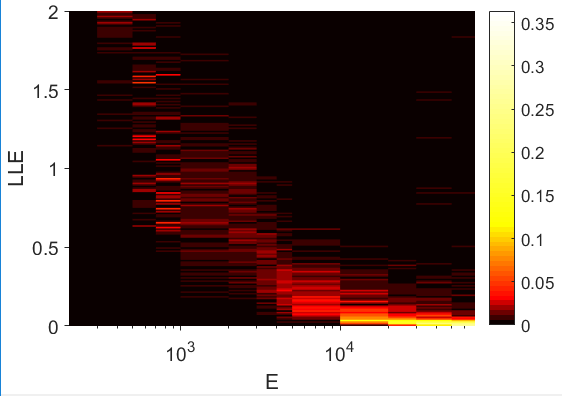
\includegraphics[scale=0.4]{ZhiyuPictures/LLEdistribution_1_11_pre_hot1_screenshot.png}
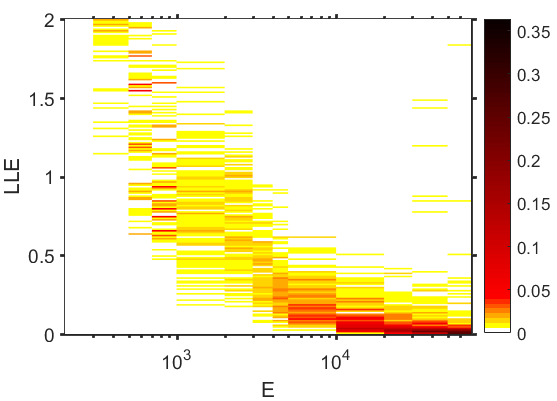
\includegraphics[scale=0.4]{ZhiyuPictures/LLEdistribution_1_11_pre_hot2_screenshot.png}
\caption{LLE distribution for N=5, F0=1000, scan E. The size of bin is 0.01}\label{fig:LLEdistribution1}
\end{figure}

%\begin{figure}[h]
%\centering
%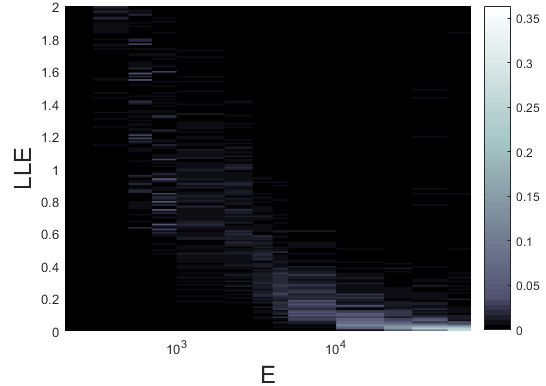
\includegraphics[scale=0.4]{ZhiyuPictures/LLEdistribution_1_11_pre_bone1_screenshot.png}
%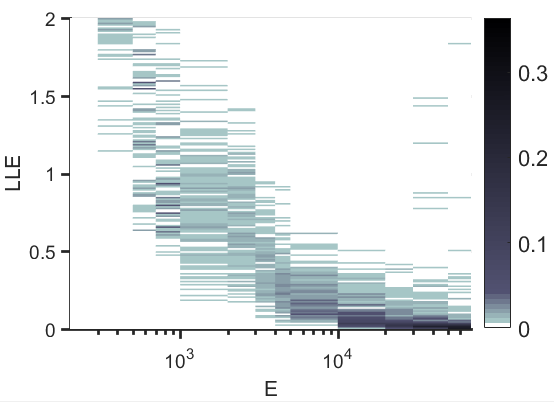
\includegraphics[scale=0.4]{ZhiyuPictures/LLEdistribution_1_11_pre_bone2_screenshot.png}
%\caption{``bone". top(bottom):modified(reversed)}
%\end{figure}


The LLE decrease with the growth of Energy. The crucial part is near E=5000. The most probable value of LLE goes down from 1 to 0.1,which indicate that the shortest time scale becomes longer than an oscillation period when E is larger than 5000, which is consistent with our prediction value of thermalization threshold. So there is a correspondence between energy thermalization and LLE. As E goes far beyond the thermalization threshold value, the LLE is restricted close to zero, suggesting the divergence of correlation time.




\section{Shape of Distribution in Phase-space}\label{section:Shape}
When describing simple harmonic motion, it is usually convenient to use the language of phase-space (of single particle). In the phase-space, the motion becomes circular, so each of these particles has two independent degrees of freedom, i.e., modulus and phase angle. Here, ``independent" means that the simple harmonic oscillation never ``mix" these two degrees of freedom. In view of this, when it comes to ``thermalization", one will expect that the thermalization of energy, which is just the modulus, does not ensure the thermalization of phase angle. As ins explained in the Introduction part, in order to distinguish two kinds of meanings of ``thermalization", we will call the process of energy distribution going to equilibrium ``thermalization", while the process of phase angle going to equilibrium ``relaxation". The time scale of thermalization and relaxation could be quite different in principle. We will start with the configuration where particles' velocities are set to be zero, which means in phase-space the cloud is a rotating narrow ellipse at the beginning. If the time scale of thermalization is much longer than that of relaxation, we will see cloud going to some stable shape in a short time (a circle if interaction is not significant compared to total energy) while the distribution of particle number along radius slowly evolves to Boltzmann distribution. If the relaxation time is longer than the thermalization time, the cloud will maintain elliptical shape or some oscillation between different shapes for a long time while the energy distribution is already Boltzmann.

To quantify the shape of distribution in phase-space, we defined a shape polarization S:
\begin{equation}
S=\frac{a-b}{a+b}
\end{equation}
where a and b are long axis and short axis of inertia ellipse in phase space respectively. a,b can be calculated by diagonalizing the inertia tensor I: $I_{xx}=\sum{p^2}, I_{xp}=I_{px}=-\sum{xp},I_{pp}=\sum{x^2}$. S=1 for line-shape distribution, S=0 for circular distribution. The advantage of defining the S lies in that S is independent of all rotating behavior of the cloud in phase-space and thus extract the information of shape alone. One could also use eigenvalues of quadrupole moment Q to define S. Two choice of definition is equivalent, since I and Q are only different up to a factor and an identity matrix.



%First, let's see the overall value of S in Fig.\ref{fig:shape}. In Fig.\ref{fig:shape}, each data point is the average of S over several periods to show the overall value of S. If the shape relax to equilibrium, the overall value should decrease to zero. At first sight, it seems S does relax, and the conclusion looks similar to the one we got from Boltzmann distribution--When energy is lower than thermalizing threshold(top pannel), S relax in almost no time; when energy is higher than thermalizing threshold(bottom pannel), it takes a relativly long time for S to relax. The reason why S never decay to zero could be explained as the contribution of random fluctuation, since S is defined to be positive.

%However, it is not the whole story. If we inspect the original data or smoothen it by taking a finer average, e.g. average over 0.2 time units (Fig.\ref), we will see the ''sinusoidal"  oscillation of S (S is defined to be positive) with a period of about $2\pi$ time units. So the whole picture is that the shape of the cloud is oscillating: \\elliptical with long axis lying along x axis $\rightarrow$ circular $\rightarrow$ elliptical with long axis lying along y axis $\rightarrow$ circular ...

%If we think of the cloud as 2D cloud in x-p space, we have 2D monopole, dipole and quadrupole mode. In our system, since energy conserves, $x^2+p^2$ is a constant interaction energy is neglected), the monopole mode do not exist. And dipole mode describes the center of mass of the cloud oscillate along x or p, but since we set center of mass to be stationary and at x=0, neither does this mode exist. The lowest order mode is quadrupole mode.

The time evolution of S is shown in Fig.\ref{fig:time_evolution_of_S}. The top three pannels are the overall value of S, where every data point is the average value of original data over several period (about $2\pi$ time unit). The lower six pannels are the original data measured in the beginning and after thousands of time units, which shows the finer structure in one period. 

\begin{figure*}[h]
\subfigure[$N=20, F_0=1000, E=3000$]{
\begin{minipage}[b]{0.3\linewidth}
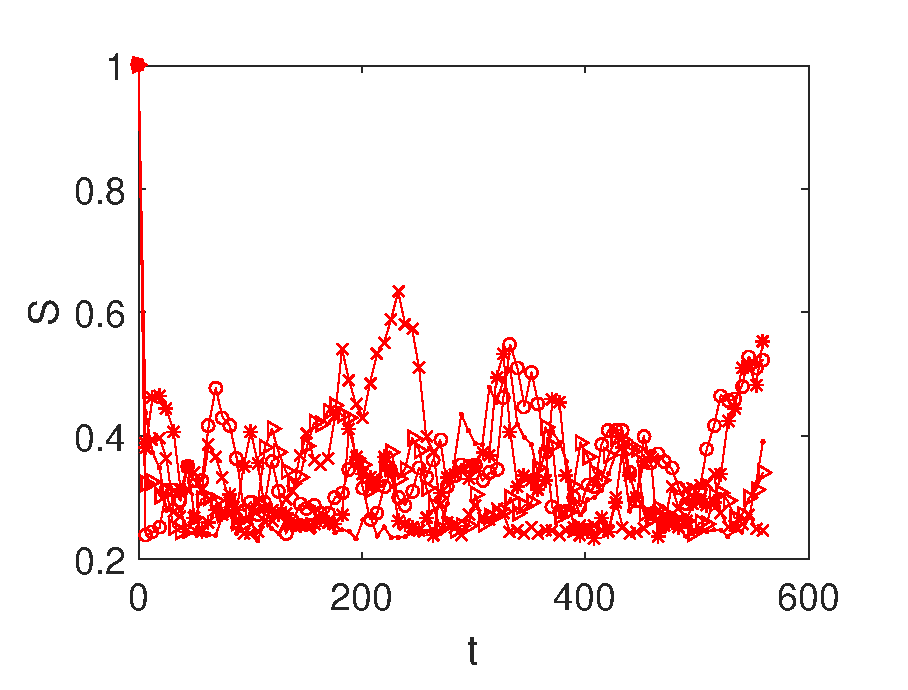
\includegraphics[scale=0.4]{ZhiyuPictures/N=20_shape_F=1000_E=3000_1.eps}
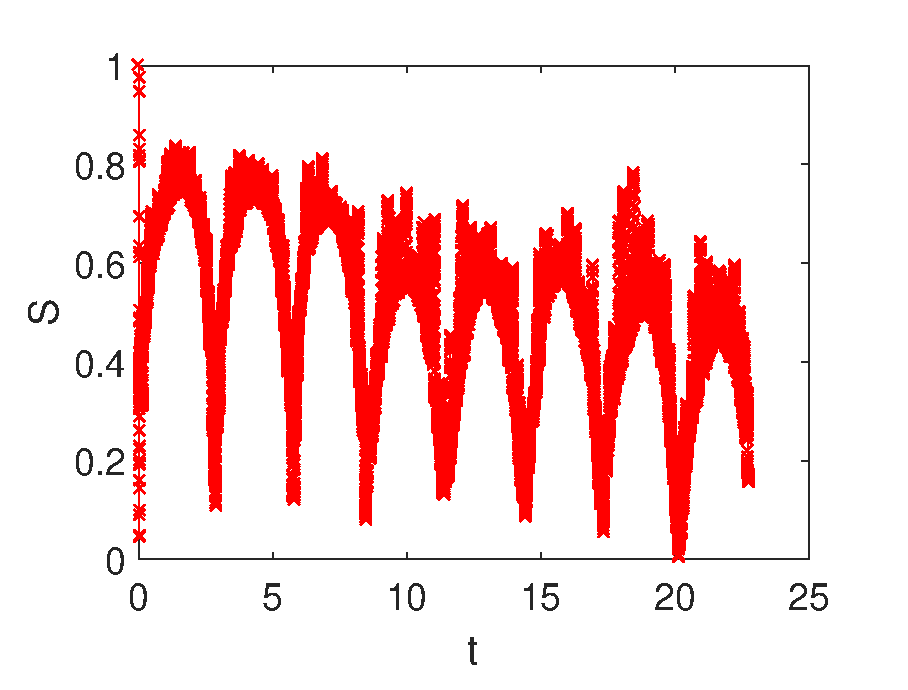
\includegraphics[scale=0.4]{ZhiyuPictures/N=20_shape_F=1000_E=3000_2_crude_begin.eps}
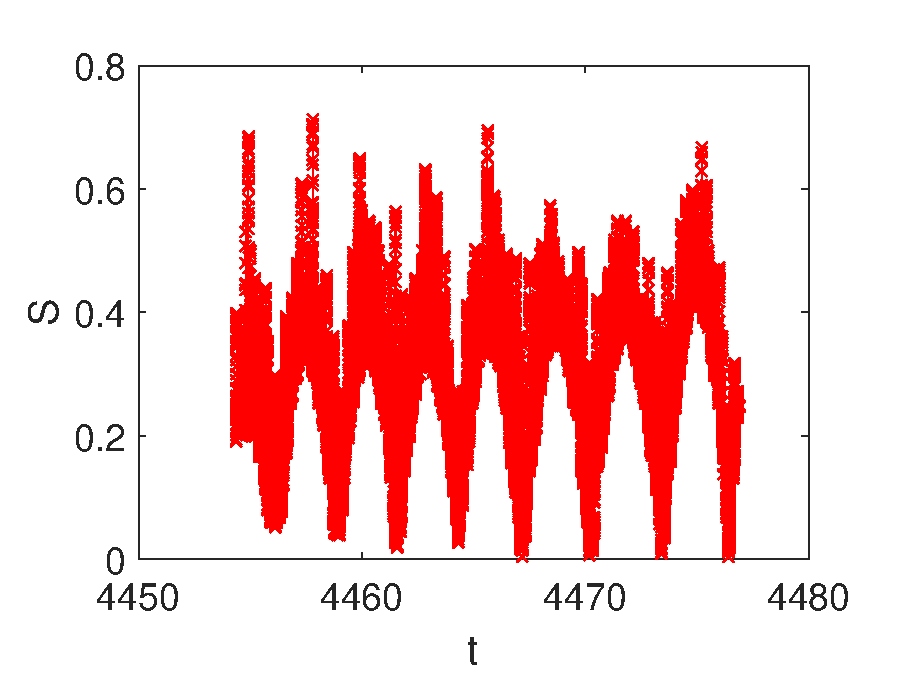
\includegraphics[scale=0.4]{ZhiyuPictures/N=20_shape_F=1000_E=3000_2_crude_end.eps}
\end{minipage}
}
\subfigure[$N=20, F_0=1000, E=20000$]{
\begin{minipage}[b]{0.3\linewidth}
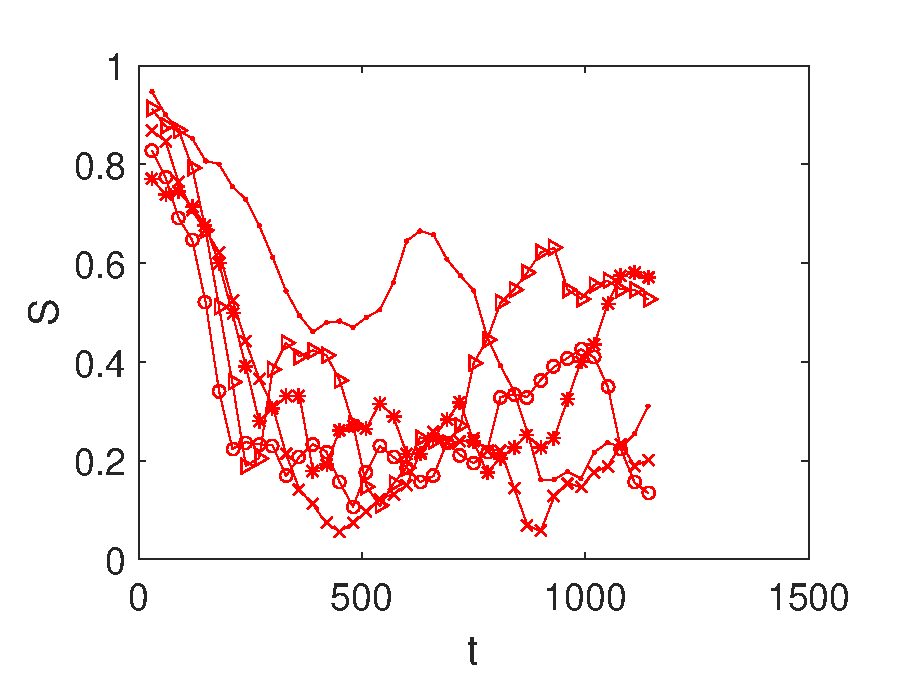
\includegraphics[scale=0.4]{ZhiyuPictures/N=20_shape_F=1000_E=20000_1.eps}
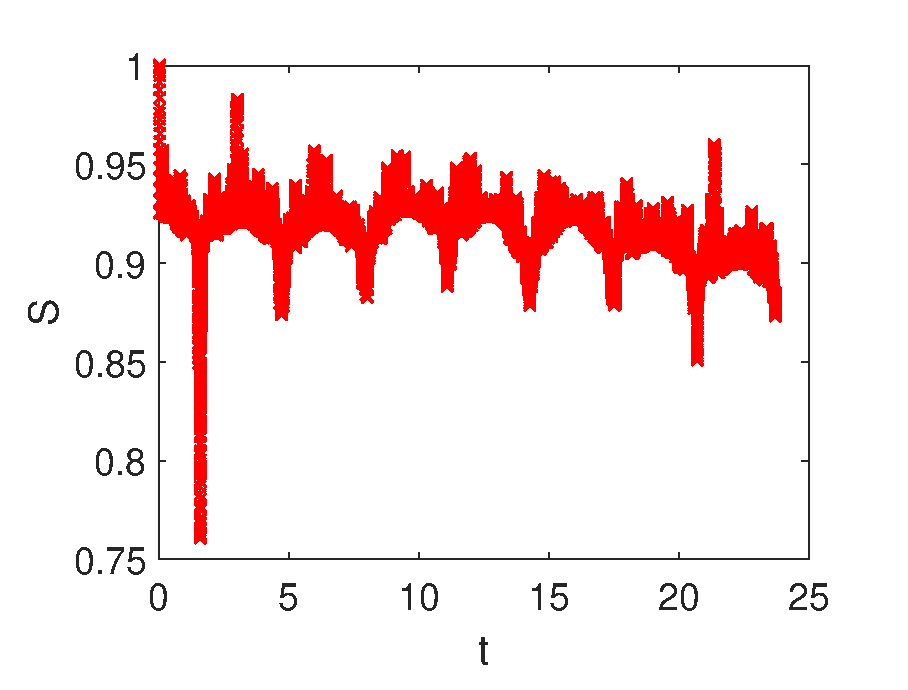
\includegraphics[scale=0.4]{ZhiyuPictures/N=20_shape_F=1000_E=20000_2_crude_begin.eps}
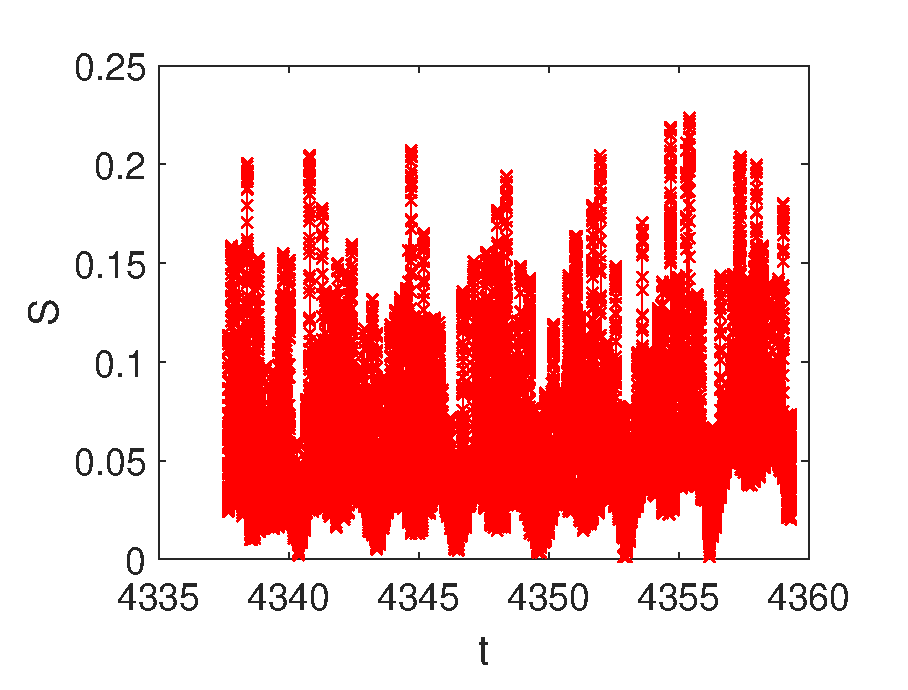
\includegraphics[scale=0.4]{ZhiyuPictures/N=20_shape_F=1000_E=20000_2_crude_end.eps}
\end{minipage}
}
\subfigure[$N=20, F_0=1000, E=100000$]{
\begin{minipage}[b]{0.3\linewidth}
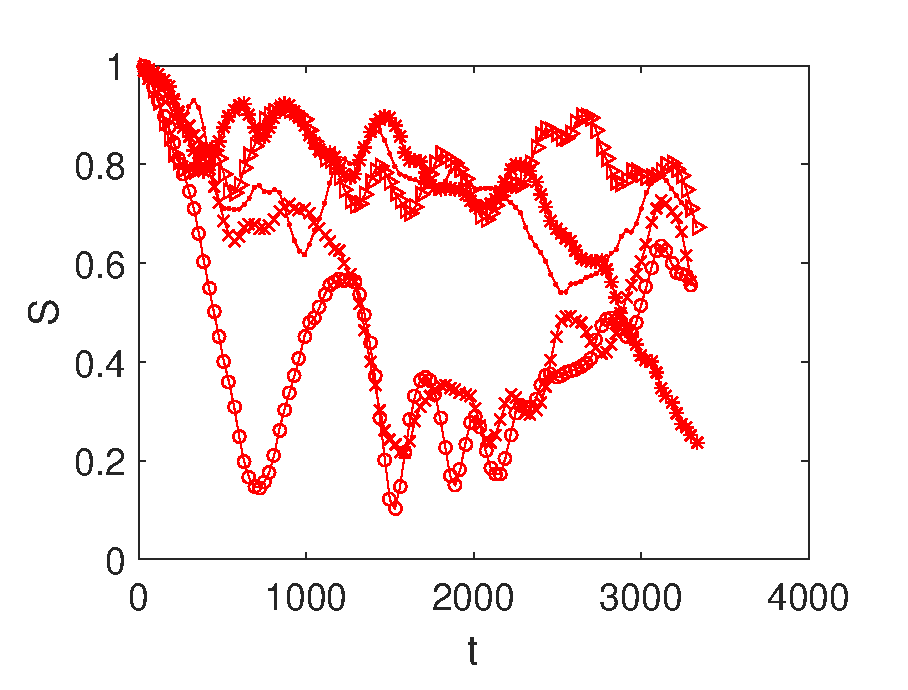
\includegraphics[scale=0.4]{ZhiyuPictures/N=20_shape_F=1000_E=100000_1.eps}
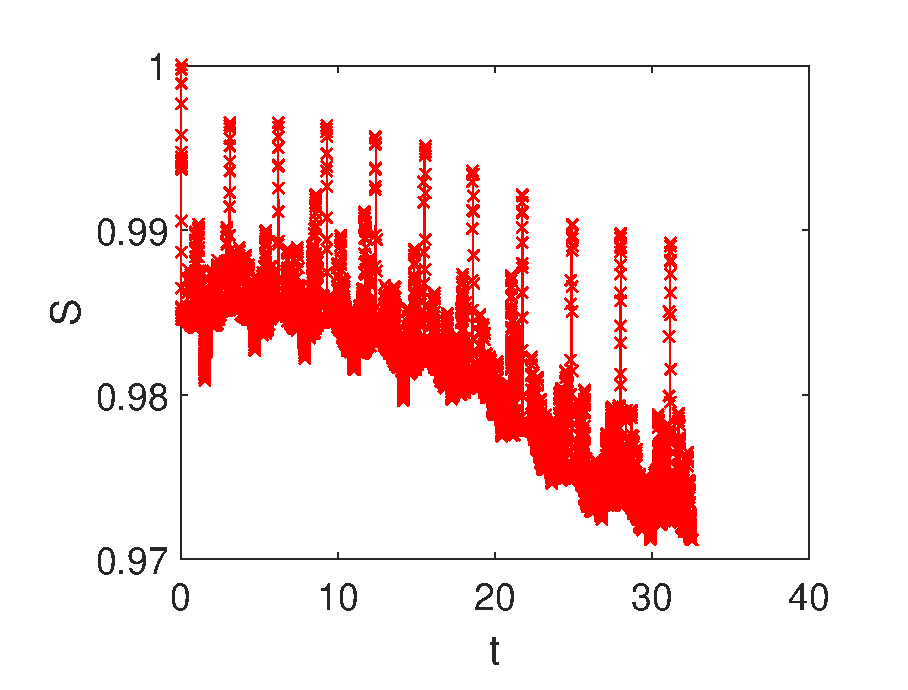
\includegraphics[scale=0.4]{ZhiyuPictures/N=20_shape_F=1000_E=100000_2_crude_begin.eps}
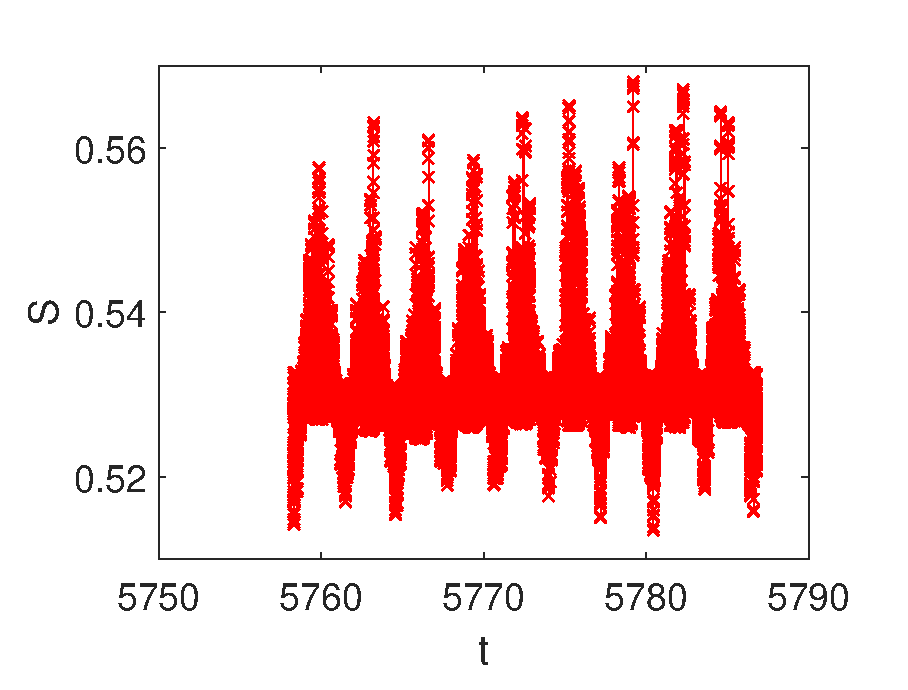
\includegraphics[scale=0.4]{ZhiyuPictures/N=20_shape_F=1000_E=100000_2_crude_end.eps}
\end{minipage}
}
\caption{Time evolution of S in low-energy regime(a), intermidiate(b), high-energy regime(c). The overall value (top three pannels), where every point represent the average of original data over several periods, show that S decays to a low value in a short time in low-energy case, but persist for a relative long time in high-energy case. The snapshots of original data at beginning and after thousands of periods evolution are shown in the lower six pannels. The finer structure of S(t) indicates that there is some long-lasting oscillating mode. Especially in low-energy case, the amplitude is more conspicuous.}\label{fig:time_evolution_of_S}
\end{figure*}

%\begin{figure}
%\centering
%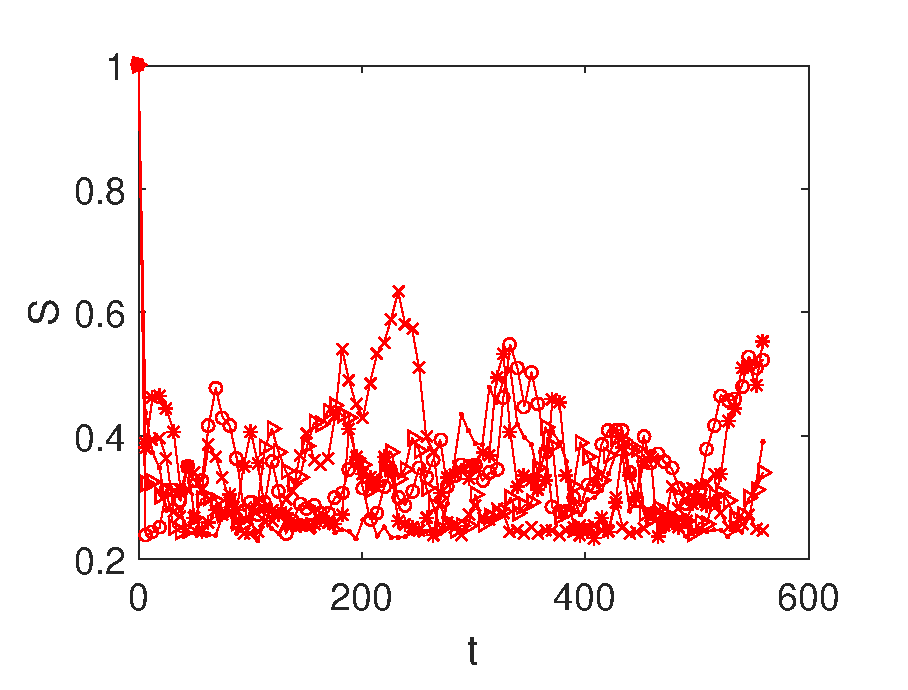
\includegraphics[scale=0.4]{ZhiyuPictures/N=20_shape_F=1000_E=3000_1.eps}
%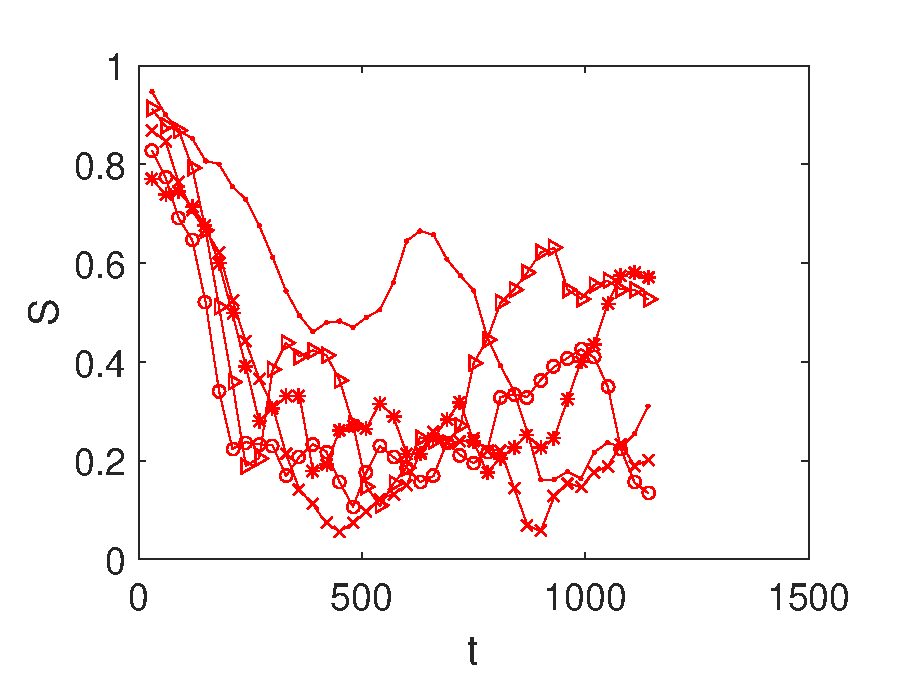
\includegraphics[scale=0.4]{ZhiyuPictures/N=20_shape_F=1000_E=20000.eps}
%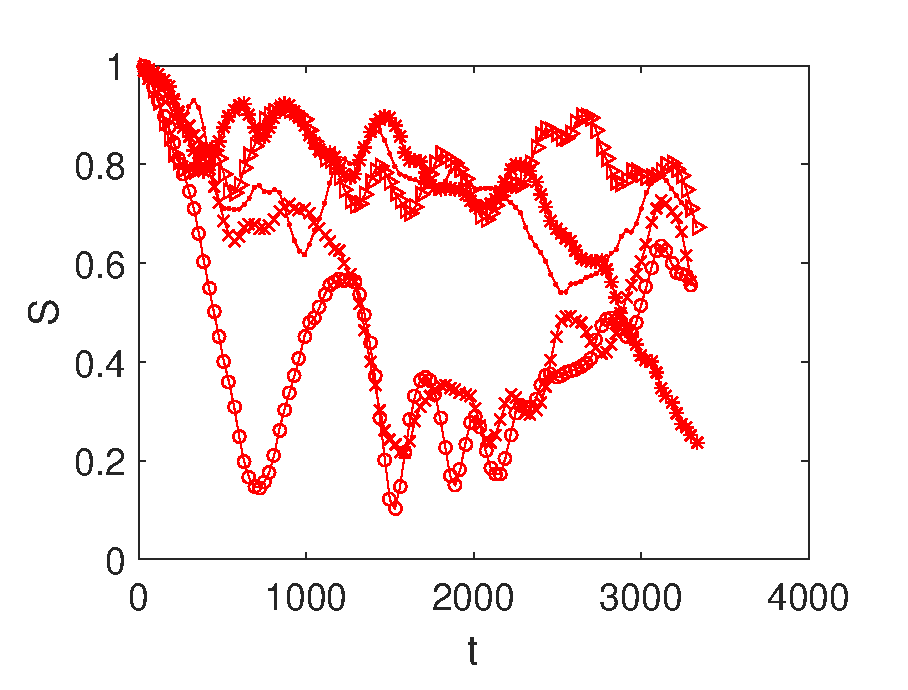
\includegraphics[scale=0.4]{ZhiyuPictures/N=20_shape_F=1000_E=100000.eps}
%\caption{N=20, F=1000, E=3000(top), E=20000(middle), E=100000(bottom). All start with initial states S=1. Five different curves in each picture represent simulating with 5 random initial states in each case. \label{fig:shape}}
%\end{figure}


%\begin{figure*}
%\centering
%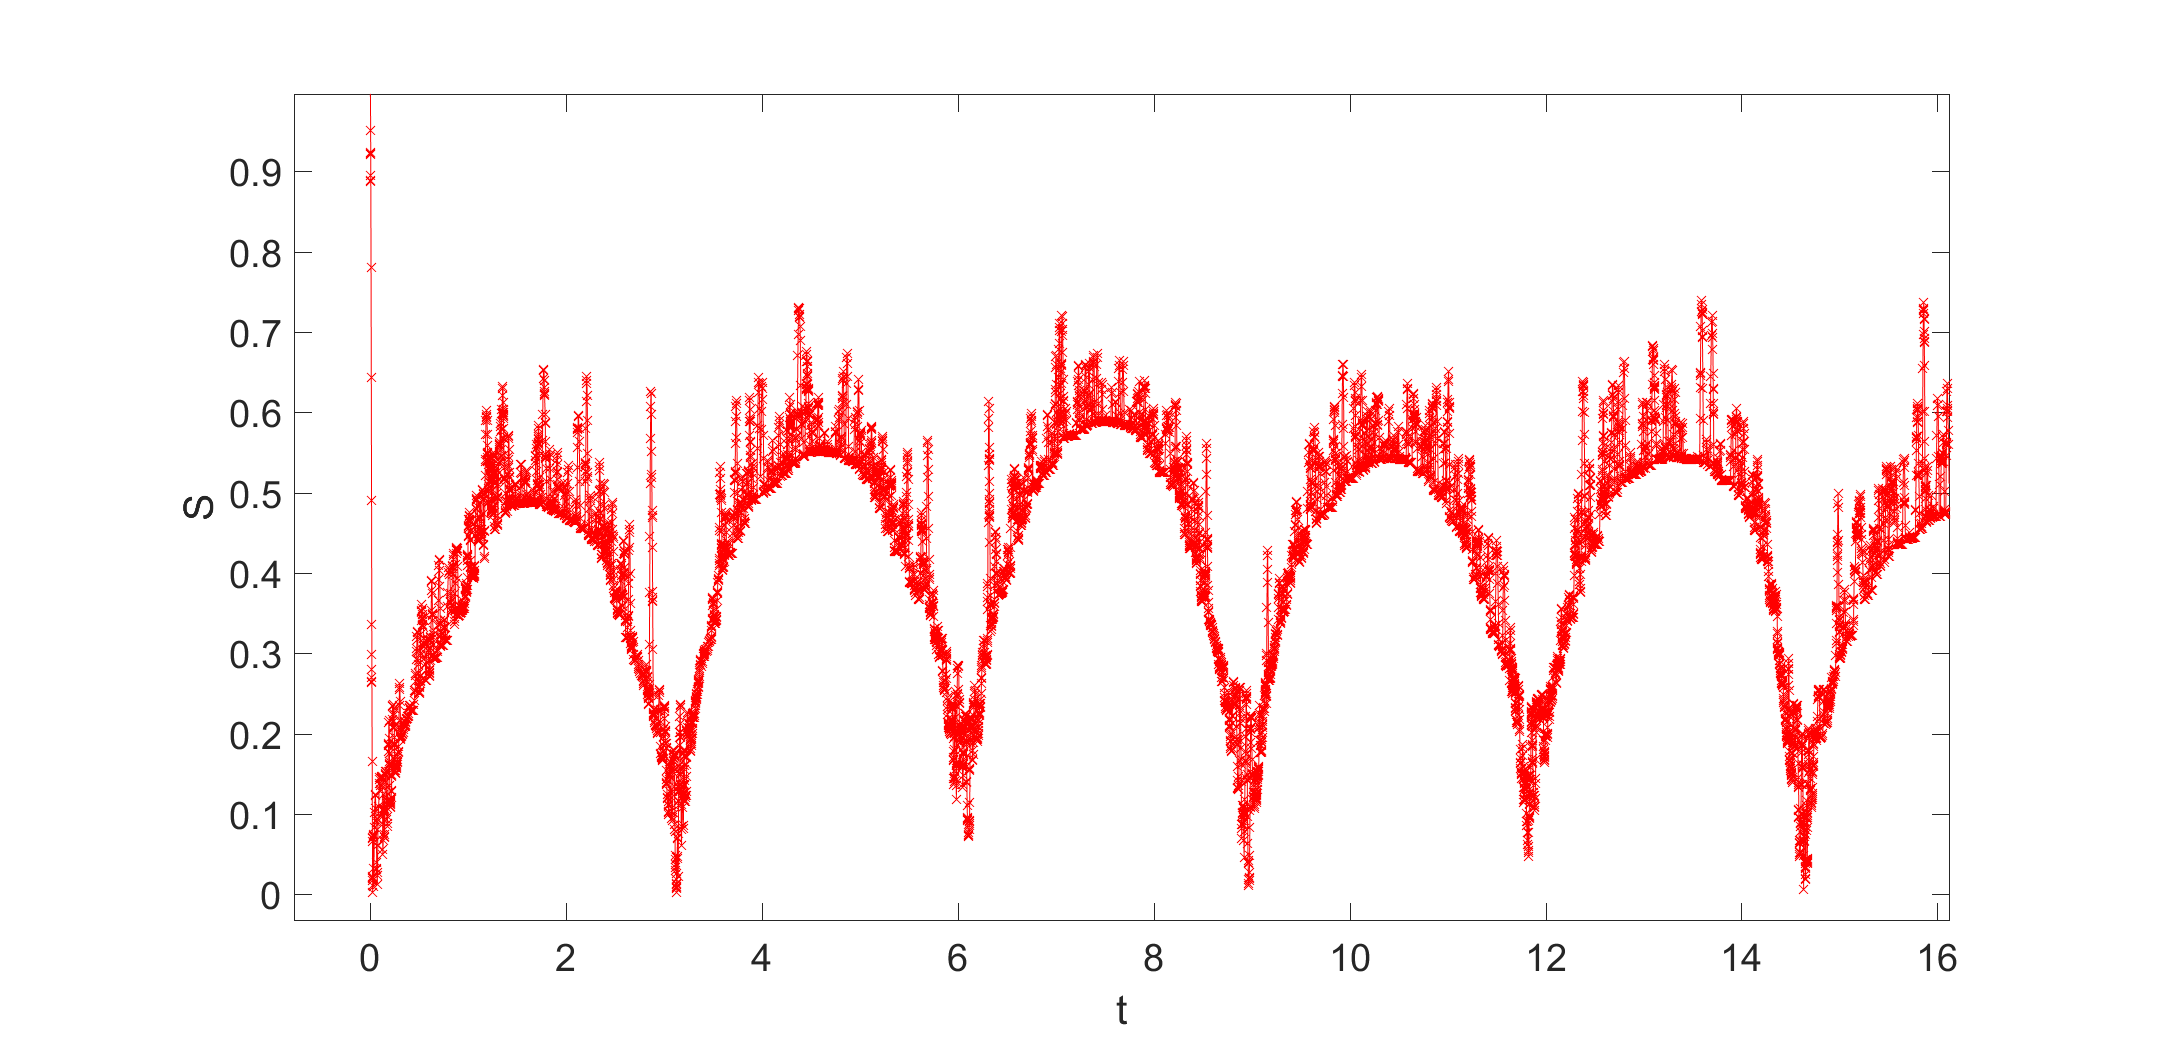
\includegraphics[scale=0.4]{ZhiyuPictures/N=20_shape_F=1000_E=3000_original1.eps}
%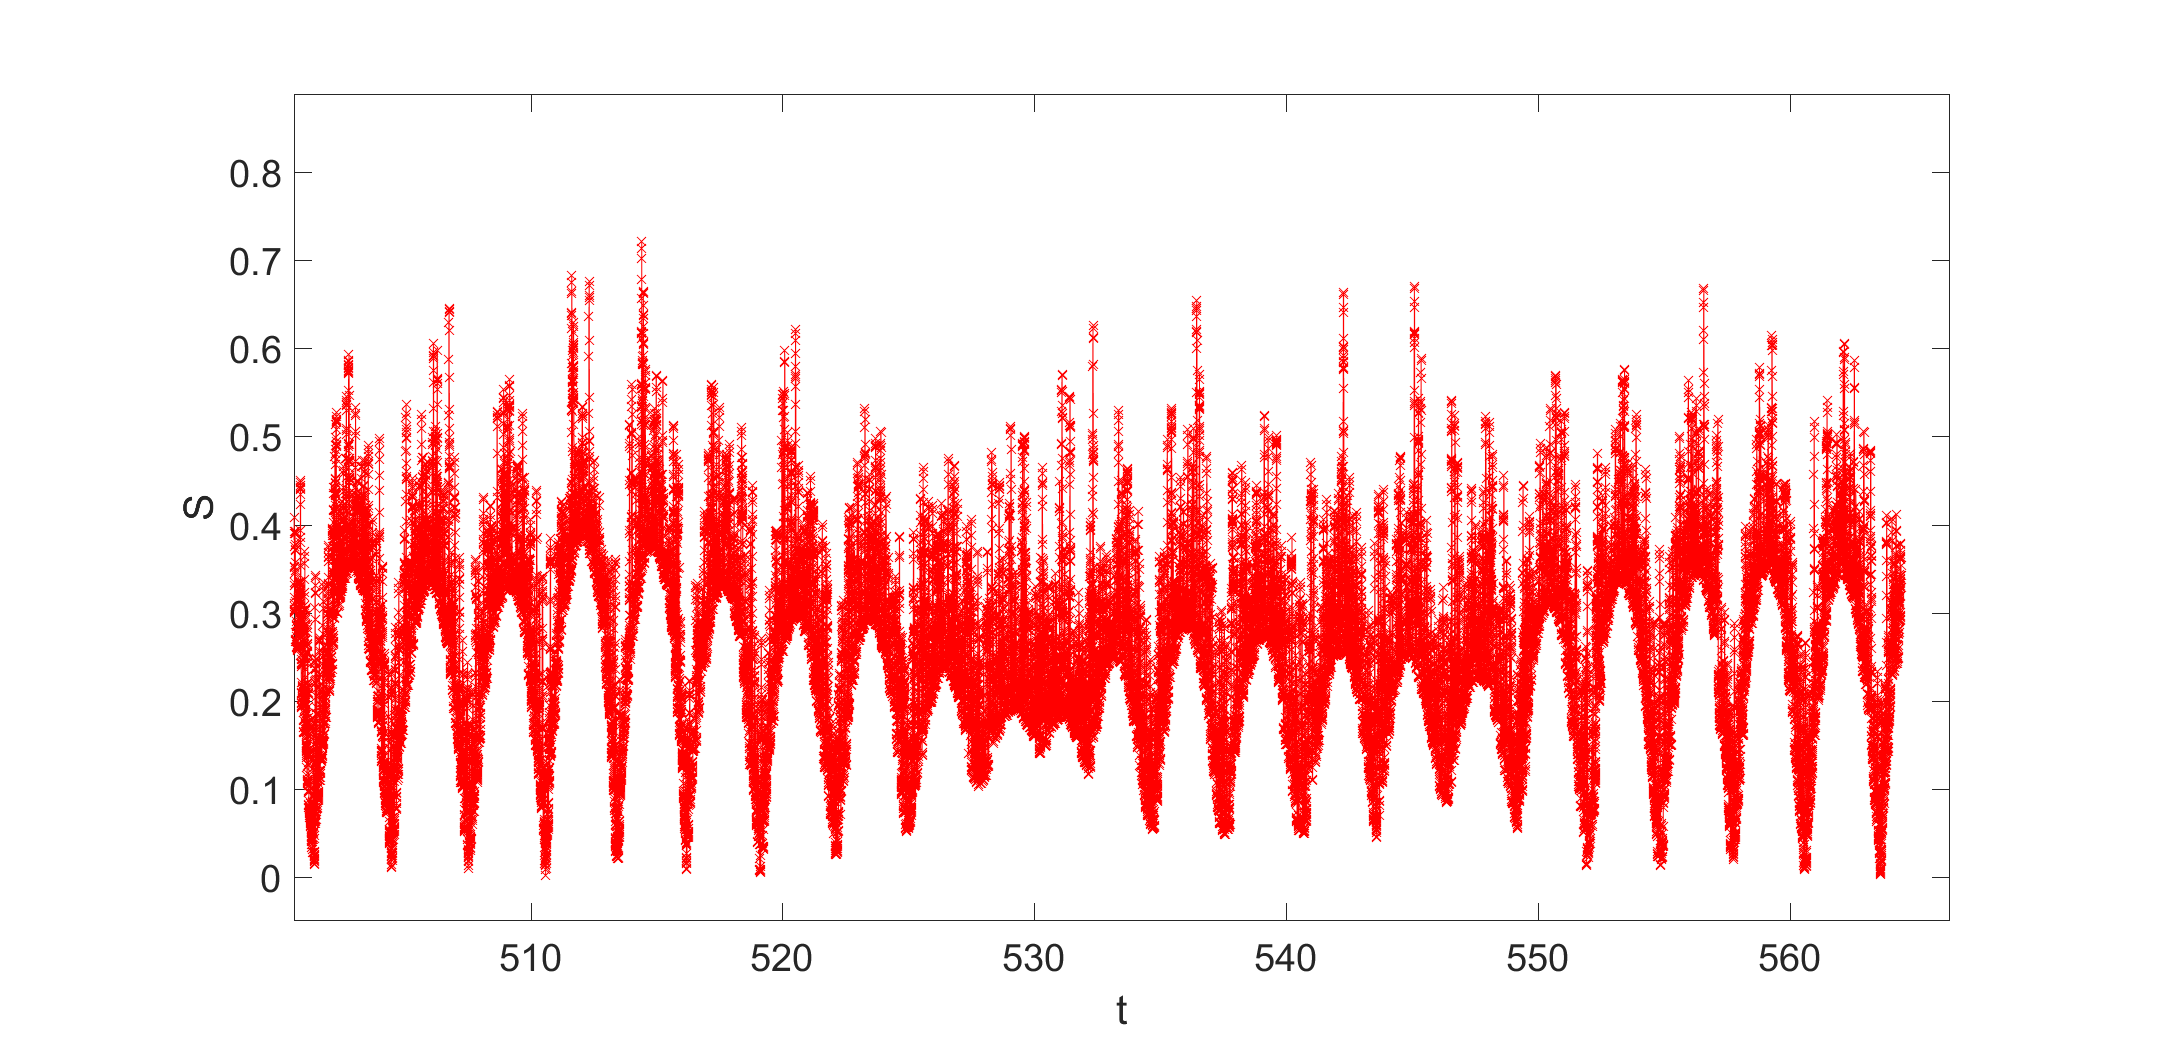
\includegraphics[scale=0.4]{ZhiyuPictures/N=20_shape_F=1000_E=3000_original2.eps}
%\caption{N=20, F=1000, E=3000. Original data}
%\end{figure*}

%\begin{figure*}
%\centering
%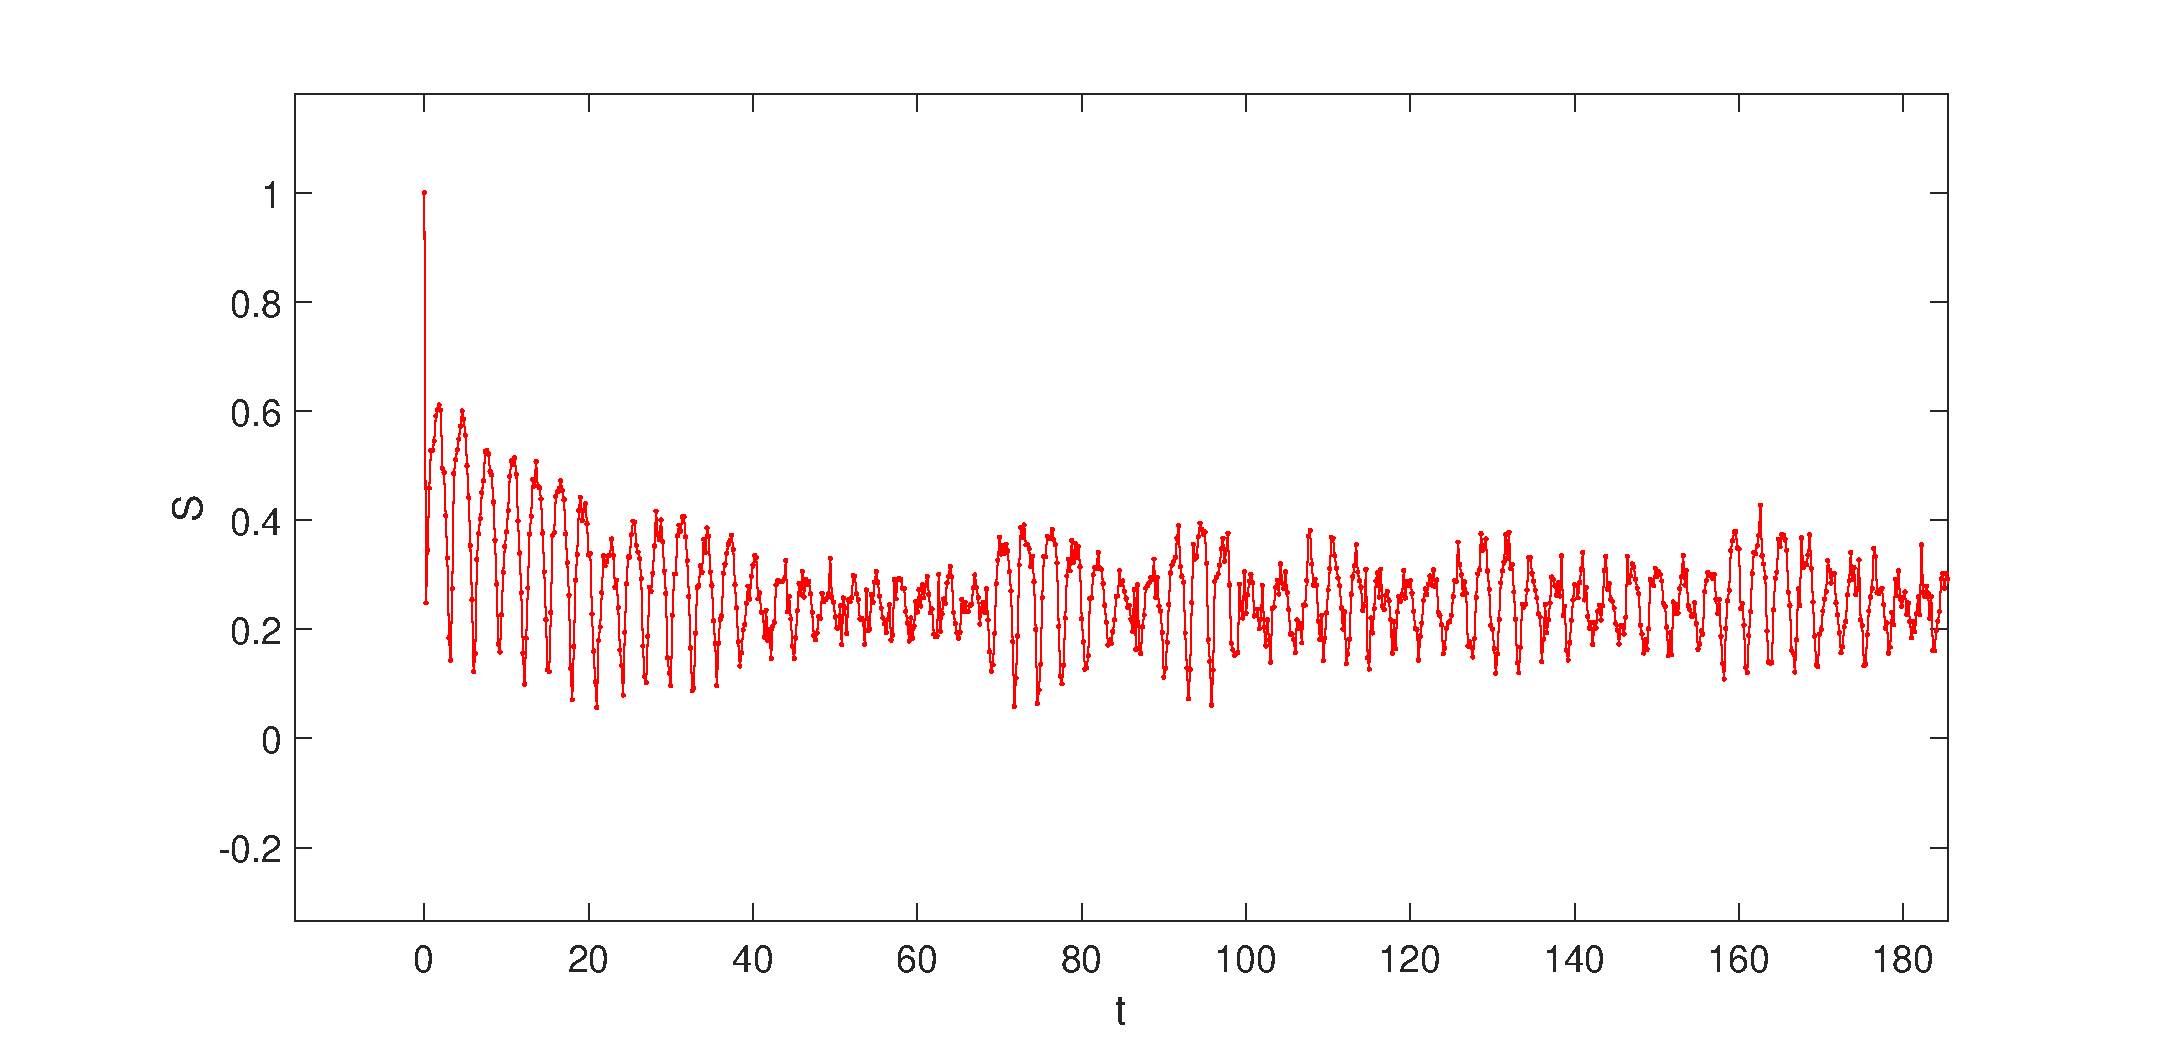
\includegraphics[scale=0.4]{ZhiyuPictures/N=20_shape_F=1000_E=3000_1_fine1.eps}
%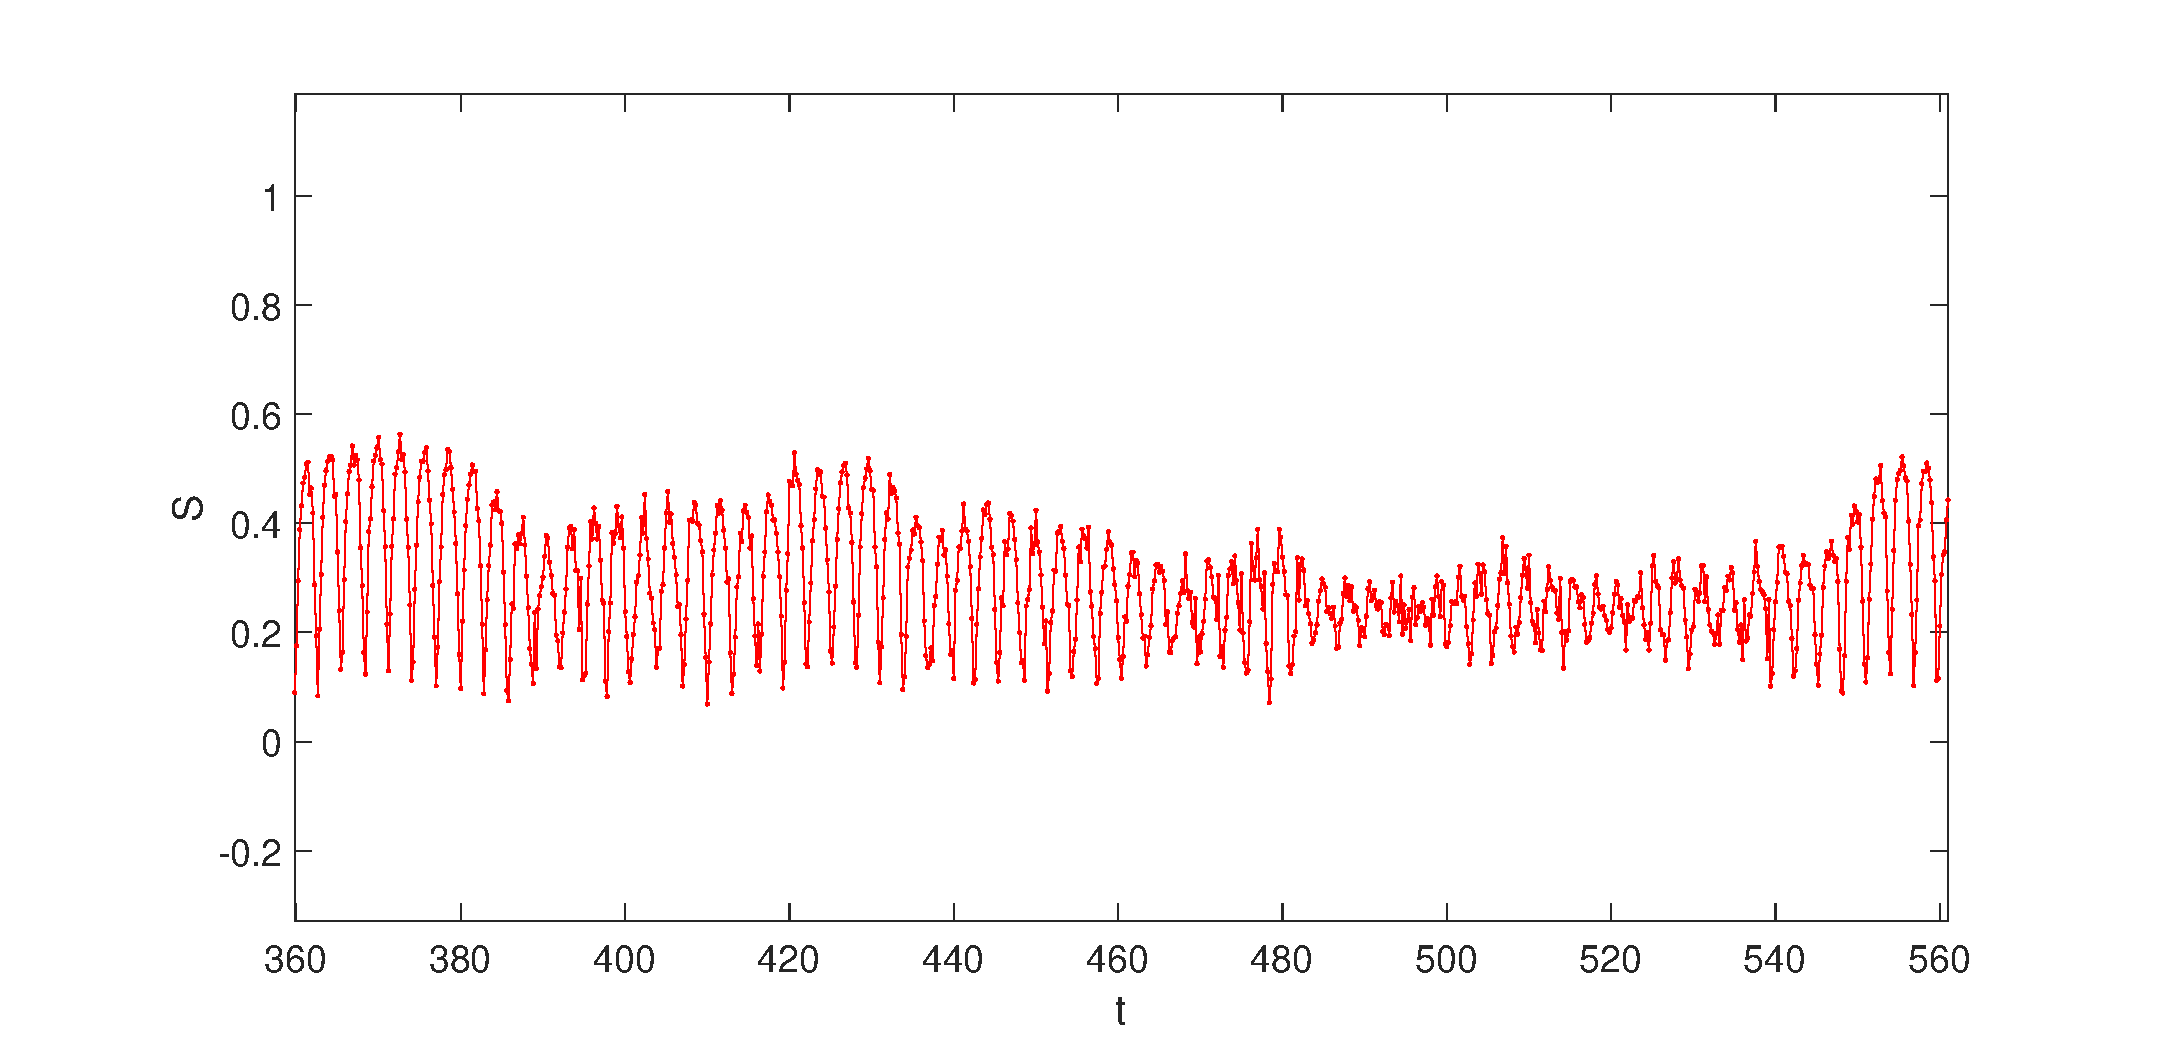
\includegraphics[scale=0.4]{ZhiyuPictures/N=20_shape_F=1000_E=3000_1_fine2.eps}
%\caption{N=20, F=1000, E=3000. Start with initial states S=1. Smoothened (every point represents taking the average of S in 0.2 time unit)}
%\end{figure*}

The original data can be decomposed into two components: the background value and the frequent fluctuation(sharp peaks and dips) on the background. The fluctuation is generated from the two-particle transportation process(See Fig.\ref{fig:Breathingfrequency3}), e.g. a pair transportation event along the long-axis of the cloud makes a dip. In the thermalized regime (Fig.\ref{fig:time_evolution_of_S}), the background value of S is oscillating with an amplitude of 0.2-0.4 and does not decay to zero over 4000 time unit. In the high-energy case, the amplitude of background oscillation is small compared with fluctuation. We assume that over a long enough time, all macroscopic quantity should be constant because the randomness has wash out all possible orders to make entropy as large as possible. Since we see a periodical behavior of S, we know the whole system doesn't relax to its equilibrium state.  

The oscillating background value of S indicate that the shape of the cloud in phase space is deformed periodically between a circle and an ellipse($S=0.4$ means $\frac{a}{b}\sim 2.5$). To further reveal the nature of this oscillating mode, we focus on the low-energy case and plot the distribution of the cloud in the phase-space as Fig.\ref{fig:N=50_F=1000_E=30000_movie}. The time interval between each pannels is $0.1*2\pi$ time units. The direction of the yellow arrows and red arrows are the eigenvector of inertia tensor, while their lengths are the square root of correspondent eigenvalue (I take the squareroot to maintain the length unit). In most of the pannels in Fig.\ref{fig:N=50_F=1000_E=30000_movie}, the long and short axis are rotating and extending or contracting continuosly. The exception is the 3rd and 4th pannel in the first row, 2nd and 3rd pannel in the second row, 1st and 2nd pannel in the third row. At those moment, the long and short axis are almost equal, giving the system a chance to choose a new preferred axis to polarize. The whole picture of this collective mode can be described by Fig.\ref{fig:Schemetic_description_of_the_mode}, which is consistant with the pattern of time evolution of S shown in Fig.\ref{fig:N=50_F=1000_E=30000_Send}.

\begin{figure*}[h]
\centering
\includegraphics[scale=0.5]{ZhiyuPictures/N=50_F=1000_E=30000_shapemovie_interval0_628_2_500s_1100_600_Font18.eps}
\caption{Distribution in phase-space after evolving for about 500 time units ($N=50, F_0=1000, E=30000$). Please notice that the yellow(red) arrows shows the length of long(short) axis of inertia ellipse, which is prependicular to the long(short) axis of distribution cloud. For instance, if the yellow arrow lies in p-axis, it means the long axis of distribution cloud is lying along x-axis.}\label{fig:N=50_F=1000_E=30000_movie}
\end{figure*}

\begin{figure*}[h]
\centering
\includegraphics[scale=0.4]{ZhiyuPictures/quadrupole_mode_2.png}
\caption{Schemetic description of the excited mode.  Red ellipse is the shape of cloud in low-energy regime when there is repulsive interaction. Gray cloud is the imaginary shape of cloud when there is no interaction, which is plotted here as a reference. One may think of the effect of interaction as a kind of potential that prefer to place particles along x axis, because in low energy regime the system is not allowed to be squeezed too much along x axis since doing this cost a large amount of interaction energy.}\label{fig:Schemetic_description_of_the_mode}
\end{figure*}

\begin{figure*}[h]
\centering
\includegraphics[scale=0.4]{ZhiyuPictures/N=50_F=1000_E=30000_shapemovie_interval0_628_2_500s_Send.eps}
\caption{Time evolution of S after evolving for about 500 time units ($N=50, F_0=1000, E=30000$). The oscillating behaviour of S persists over 500 time units.}\label{fig:N=50_F=1000_E=30000_Send}
\end{figure*}

To sum up, the existence of the long-lasting oscillation of S indicate that the system does not relax to its equilibrium state in terms of shape although it is already thermalized in terms of energy distribution. With this long-lasting mode, the radius R of the cloud will keep oscillating, enabling the breathing mode to last for a long time.

\section{Conclusion}
We studied the nonequilibrium property of one-dimensional classical gas with finite range repulsive interaction. We first studied the relation between breathing mode frequency and interaction parameter as well as total energy. We found the breathing frequency could be estimated by eq.\ref{eq:breathingfrequency1}. And the mechanism behind this relation is that the momentum transfer which happens instantly in collision saves the particles some time from traveling this distance. So the physics is completely the same as hardcore particle.
We found that the thermalization behavior is controlled by the competition between the interaction strength and the average energy. We point out that there could be two independent time scales in simple harmonic system in principle. One of them corresponds to the relaxation time of the energy distribution. The other one corresponds to the relaxation time of the angular distribution in phase space, which will determine the decay rate of the amplitude of the breathing mode. We have shown that in the low-energy regime, although the energy distribution reach Boltzmann distribution within several periods of oscillation, the shape keep oscillating for thousands of periods.
%However, with the form of interaction we used, i.e. finite range constant repulsive force, we found those two time scales diverge only when interaction vanish, which is a trivial singular point. In addition, the relaxation behavior of the angular distribution and radial distribution in phase space are similar. We attribute it to the fact that there is no essential bias between angular and radial transfer in phase-space for this simple form of interaction. The shortest time scale is verified numerically by Largest Lyapunov Exponent. A further question could be asked is whether there is a subtle form of interaction that could give those two time scales essentially different behavior. The observation of two different time scales in one system would be interesting.



%\begin{comment}
%\section{others(those I haven't organized it into the text in logical order but may be useful)}

%\subsection{Evolution of $R(t)$ and $\sqrt{\delta^2R(t)}/R(t)$} 
%Results are shown in Fig.\ref{fig:others1}

%\begin{figure}[h]

%\centering
%\includegraphics[scale=0.3]{D:/matlab2016/MolecularDynamics/figure/fluc_of_R_with_time2.eps}
%\caption{fluctuation of R with time }
%sigma=0.01(short range), $F_0=0.1(black), 1(blue), 10(green) ,100(red)$
%\label{fig:others1}
%\end{figure}


%\subsection{Detailed discussion of two-particle motion}
%{\color{red}{This chapter previously follow the subsection ``two-particle case" in subsection ``Dynamics study" in section ``Thermalization". But then I found we haven't used these result. So I put it at the end for the time being}}.
  

%From now on, let's stand in the the frame of center of mass to observe the motion of two-particle system. In this frame, without interaction, we will find two particles sitting symmetrically in an equivalent harmonic trap (black curve), whose shape is identical to the trap we see in the static frame. As a result, there frequency of relative motion is exactly $2\omega$(since two particle are identical). We label the position of center of mass as 0. And we may only analyze the motion on positive axis since positive and negative are symmetric. 

%Now, let's consider the interaction between them. Because of interaction, the potential curve between $+-\frac{\sigma}{2}$ should be modified to another parabolic curve that simultaneously satisfies the following two condition:\\
%1) intersect with black curve at $+-\frac{\sigma}{2}$\\
%2) minima is $+-\frac{F_0}{m\omega_0^2}$, which comes from a simple harmonic oscillator with an extra constant force $F_0$\\
%Thus, it is obvious that by comparing $\frac{F_0}{m\omega_0^2}$ and $\sigma$, we can at least divide our parameter into several regime:\\
%1) When $\frac{F_0}{m\omega_0^2\sigma}>0.5$, we will have the blue curve (see figure \ref{fig:thermalization2})\\
%2) When $\frac{F_0}{m\omega_0^2\sigma}<0.5$, the red curve\\
%3) When $\frac{F_0}{m\omega_0^2\sigma}=0.5$, the green one.\\
%For those three types of curve, the significant difference is only at low energy case:\\
%For the red one, particle will oscillate at constant frequency $\omega$;
%For the blue one, when energy is lower, since the first derivative of the curve in the neighbourhood is non-zero, the frequency goes to infinity;
%For the green curve, in low energy limit, it takes finite time to finish half period of oscillation, while infinitesimal time is spent on the slope part. Thus, frequency will converge to  $2\omega$.

%\begin{figure}
%\subfigure[]{
%\begin{minipage}[b]{0.3\textwidth}
%\includegraphics[scale=0.17]{ZhiyuPictures/freq_scanE_1.png} 
%\end{minipage}
%}
%\subfigure[]{
%\begin{minipage}[b]{0.3\textwidth}
%\includegraphics[scale=0.17]{ZhiyuPictures/freq_scanE_2.png} 
%\end{minipage}
%}
%\subfigure[]{
%\begin{minipage}[b]{0.3\textwidth}
%\includegraphics[scale=0.17]{ZhiyuPictures/freq_scanE_3.png} 
%\end{minipage}
%}
%\centering
%\caption{Frequency of relative motion with internal energy in three regime} Numbers in the legend is the value %of $\frac{F_0}{m\omega_0^2\sigma}$
%\label{fig:thermalization3}
%\end{figure}
%\end{comment}



%\bibliography{mybib}
%\bibliographystyle{ieeetr} 



\begin{thebibliography}{1}

\bibitem{Dalfovo1997}
F.~Dalfovo, S.~Giorgini, M.~Guilleumas, L.~Pitaevskii, and S.~Stringari,
  ``Collective and single-particle excitations of a trapped bose gas,'' {\em
  Phys. Rev. A}, vol.~56, pp.~3840--3845, Nov. 1997.

\bibitem{Jin1996}
D.~S. Jin, J.~R. Ensher, M.~R. Matthews, C.~E. Wieman, and E.~A. Cornell,
  ``Collective excitations of a bose-einstein condensate in a dilute gas,''
  {\em Phys. Rev. Lett.}, vol.~77, pp.~420--423, July 1996.

\bibitem{Dalfovo1999}
F.~Dalfovo, S.~Giorgini, L.~P. Pitaevskii, and S.~Stringari, ``Theory of
  bose-einstein condensation in trapped gases,'' {\em Rev. Mod. Phys.},
  vol.~71, pp.~463--512, Apr. 1999.

\bibitem{Stringari1996}
S.~Stringari, ``Collective excitations of a trapped bose-condensed gas,'' {\em
  Phys. Rev. Lett.}, vol.~77, pp.~2360--2363, Sept. 1996.

\bibitem{Haller2009}
E.~Haller, M.~Gustavsson, M.~J. Mark, J.~G. Danzl, R.~Hart, G.~Pupillo, and
  H.-C. Nägerl, ``Realization of an excited, strongly correlated quantum gas
  phase,'' {\em Science}, vol.~325, p.~1224, Sept. 2009.

\bibitem{Guery-Odelin1999}
D.~Gu\'ery-Odelin, F.~Zambelli, J.~Dalibard, and S.~Stringari, ``Collective
  oscillations of a classical gas confined in harmonic traps,'' {\em Phys. Rev.
  A}, vol.~60, pp.~4851--4856, Dec 1999.

\bibitem{Tsuchiya2000}
T.~Tsuchiya and N.~Gouda, ``Relaxation and lyapunov time scales in a
  one-dimensional gravitating sheet system,'' {\em Phys. Rev. E}, vol.~61,
  pp.~948--951, Jan. 2000.

\bibitem{Yawn1997}
K.~R. Yawn and B.~N. Miller, ``Ergodic properties and equilibrium of
  one-dimensional self-gravitating systems,'' {\em Phys. Rev. E}, vol.~56,
  pp.~2429--2436, Sept. 1997.

\bibitem{Jin2013}
F.~Jin, T.~Neuhaus, K.~Michielsen, S.~Miyashita, M.~A. Novotny, M.~I.
  Katsnelson, and H.~D. Raedt, ``Equilibration and thermalization of classical
  systems,'' {\em New Journal of Physics}, vol.~15, no.~3, p.~033009, 2013.

\end{thebibliography}




 \end{document}
